% Pro kompilaci po částech (viz projekt.tex), nutno odkomentovat a upravit
%\documentclass[../projekt.tex]{subfiles}
%\begin{document}

% moje prikazy
%\paragraph{První část -- Jaký se řeší problém? Jaké je téma? Jaký je cíl textu?}
%\bigskip
%\noindent
%\bf hruhym \it kurzivou \tt strojovo \rm zpět na normál 
%\footnote{Desktop publishing (DTP) -- tvorba tištěného dokumentu na počítači.}
%\mbox{Internet}

%bakalárska práca - technická správa
%téma: Longboard s elektrickým pohonom

\chapter{Úvod}\label{uvod}

Longboard, dlhší skateboard, je dobre známé športové vybavenie, ktoré je okrem svojho športového využitia, dnes často využívané aj ako dopravný prostriedok. 
Uplatnenie nachádza najmä v~mestách a na prepravu pri krátkych vzdialenostiach, kedy je jazda na longboarde rýchlejšia a pohodlnejšia ako pešia chôdza. 
Podobne ako pri bicykloch, kolobežkách a iných dopravných prostriedkoch, aj pri longboardoch sa objavuje trend elektrifikácie. 
Elektrický pohon umožňuje jazdu na dlhšie vzdialenosti, jazdu do kopcov, jazdu vo vyššej rýchlosti, či dokonca, pri vhodnej úprave longboardu, jazdu v~miestach, kde by jazda na klasickom longboarde bola náročná alebo nemožná.
Oproti bicyklom či kolobežkám, longboard nemá žiadne riadidlá, kde by sa mohla nachádzať brzda alebo regulátor rýchlosti, a tak je nutné mať iný spôsob ovládania. 
Na trhu sa nachádza množstvo rôznych elektrických longboardov, ktoré sa líšia výkonom, cenou, dizajnom, ale všetky majú spoločný prvok --- ovládanie pomocou bezdrôtového ovládača.
Bezdrôtový ovládač funguje veľmi dobre ako jednoduchý spôsob ovládania, ale zároveň to pri pravidelnom používaní vytvára praktické problémy.
Ovládač je nutné mať vždy so sebou a dostatočne nabitý na to, aby sa dal longboard ovládať.
Naskytá sa teda otázka, či by nebolo možné ovládať longboard aj pomocou zaSriadenia, ktoré má človek vždy so sebou --- mobilného telefónu.
To by umožnilo používať longboard aj v~prípade, ak by si človek zabudol ovládač, alebo ak by bol ovládač vybitý.
Trh v~súčasnosti ponúka longboardy s~elektonickým pohonom, ktoré umožňujú spojenie s~mobilným telefónom, avšak len na základné nastavenie a sledovanie údajov.

Táto práca sa zameriava na vývoj riadiaceho systému pre longboard s~elektrickým pohonom, ktorý umožňuje bezdrôtové ovládanie pomocou bezdrôtového ovládaču alebo mobilnej aplikácie.
Cieľom práce je vytvoriť funkčný prototyp longboardu s~elektrickým pohonom, ktorý bude spracovávať dáta zo senzorov, prispôsobovať riadenie motorov a komunikovať s~užívateľom získané dáta pomocou mobilnej aplikácie.
Neodbytnou súčasťou práce je aj analýza a testovanie bezpečnosti používania longboardu s~elektrickým pohonom, aby sa predišlo nebezpečným situáciám pri jazde.

\bigskip

V~kapitole~\ref{struktura} je popísaná štruktúra longboardu s~elektrickým pohonom, kde sú podrobne popísané jednotlivé časti zariadenia, ich úlohy a vlastnosti.
Sprostredkováva tak základné informácie o~tom, ako funguje longboard s~elektrickým pohonom a aké sú jeho možnosti.
Kapitola~\ref{analyza_trhu} sa zaoberá analýzou trhu s~elektrickými longboardmi, kde sú zhrnuté dostupné riešenia a ich výhody a nevýhody.
Na základe získaných informácií sú v~kapitole~\ref{navrh} navrhnuté technické a programové prostriedky pre konštrukciu longboardu s~elektrickým pohonom, jeho ovládanie a monitorovanie.
Je navrhnutá architektúra a princíp činnosti systému, ktorý umožňuje bezdrôtové ovládanie longboardu pomocou mobilnej aplikácie.
%TODO: neskor doplniť ostatné kapitoly

\chapter{Štruktúra longboardu s~elektrickým pohonom}\label{struktura}

Longboard s~elektrickým pohonom sa skladá z~niekoľkých hlavných častí: napájanie, pohon, ovádanie a monitorovanie.
Každá z~týchto častí má svoje špecifické vlastnosti a úlohy, ktoré sú dôležité pre správne fungovanie zariadenia.\cite{WikiElectricSkateboard}

\section{Pohon}
Pohon je súbor zariadení, ktoré podľa zadaných vstupov prevádza energiu z~napájania na pohyb kolies.
Z~obyčajného longboardu sú to nohy jazdca, ktoré tlačia a brzdia longboard, ale v~prípade elektrického longboardu je to elektromotor, ktorý poháňa kolesá.

\subsection{Elektromotor}
Motor je stroj, ktorý prevádza elektrickú energiu na mechanickú.
Existuje niekoľko typov elektromotorov, ktoré sa líšia v~spôsobe fungovania, konštrukcii a vlastnostiach.
Medzi najpoužívanejšie typy elektromotorov v~odvetví elektromobility patria:
\begin{itemize}
    \item {DC (Direct Current) motor}
    \item {BLDC (Brushless Direct Current) motor}
\end{itemize}
Zvyčajne sú to však BLDC motory, ktoré sú preferované v~modelárstve a elektromobilite pre svoje vlastnosti.
Ponúkajú vysoký výkon, efektivitu, nízku údržbu a dlhú životnosť.
BLDC motory sú bezkomutátorové motory, ktoré majú viac vinutí a permanentné magnety na rotoroch.
Tieto motory vyžadujú elektronický spínač, ktorý riadi prúd vinutím a tým aj smer a rýchlosť otáčania motora.\cite{Teja}

\bigskip

Spojenie samotného motora a kolies na truckoch longboardu môže byť realizované niekoľkými spôsobmi.
Každý spôsob má svoje výhody a nevýhody, ktoré je potrebné zvážiť pri výbere vhodného riešenia.

\newpage

\subsubsection{Belt (Gear) drive}
Belt drive je spôsob pohonu, kedy je motor umiestnený mimo kolesá a poháňa ho pomocou remeňa alebo reťaze (\ref{fig:belt-drive}).
Tento spôsob umožňuje ľahkú výmenu motora alebo kolies a aj možnosť použitia prevodov.
Nevýhodou je vyššia hmotnosť a komplexnosť systému, ktorá môže viesť k~väčšiemu opotrebeniu a poruchám.
Väčšie množstvo pohyblivých častí môže tiež viesť k~vyššiemu hluku a nižšej efektivite.\cite{WikiElectricSkateboard}

\begin{figure*}[h]
    \centering
    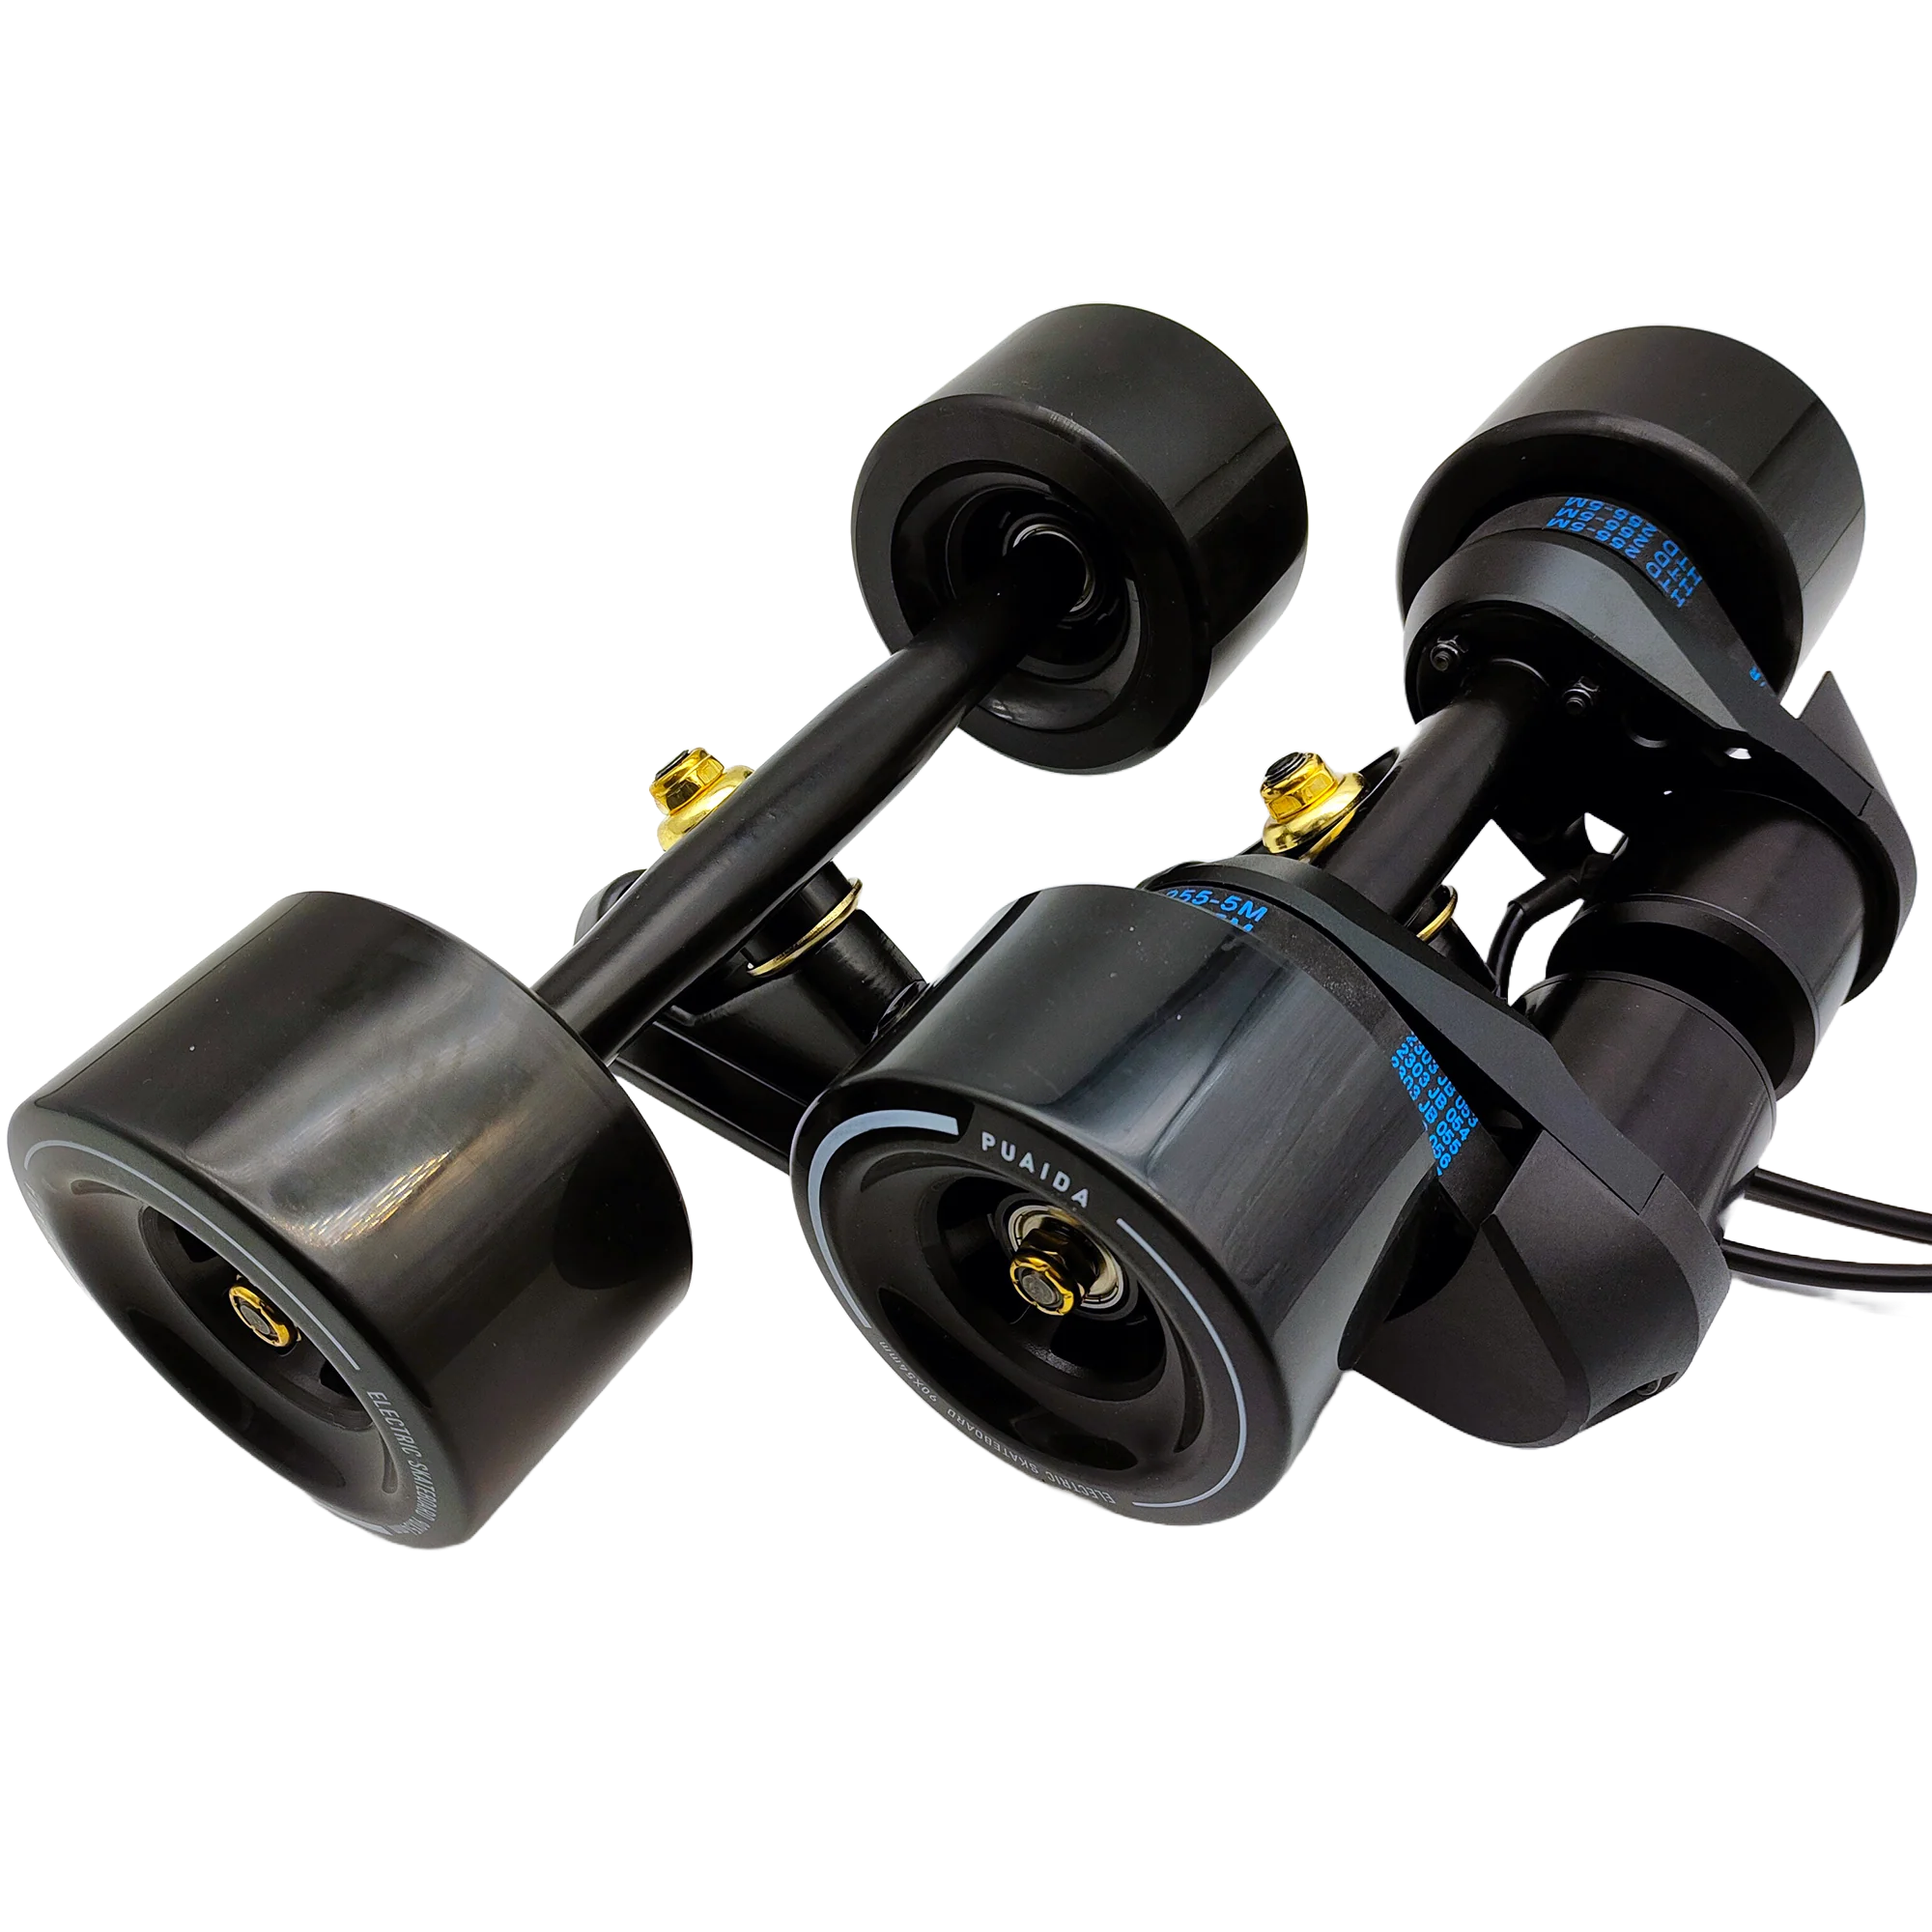
\includegraphics[height=8cm, width=1\linewidth, keepaspectratio]{obrazky-figures/drive-belt.png}
    \caption{Belt drive pohon\cite{Puaida}}\label{fig:belt-drive}
\end{figure*}

\subsubsection{Hub motor drive}
Hub motor drive je spôsob pohonu, pri ktorom je motor umiestnený priamo v~kolesách (\ref{fig:hub-drive}).
Veľkou výhodou je tichý chod a jednoduchosť pre montáž a údržbu. 
Tieto výhody so sebou prinášajú rovnako veľké nevýhody.
Uzavretá konštrukcia motoru môže pri vyššom výkone spôsobovať prehriatie a tým aj k~zníženie životnosti motora. 
Vzhľadom na to, že motor je priamo v~kolesách, je nemožné ho vymeniť bez výmeny celého kolesa, pokiaľ by nový motor od iného výrobcu.
Rovnako je ťažšie použiť kolesá od iných výrobcov, ktoré by mohli mať iné vlastnosti, ako napríklad väčší priemer alebo iný tvar.\cite{WikiElectricSkateboard}

\begin{figure*}[h]
    \centering
    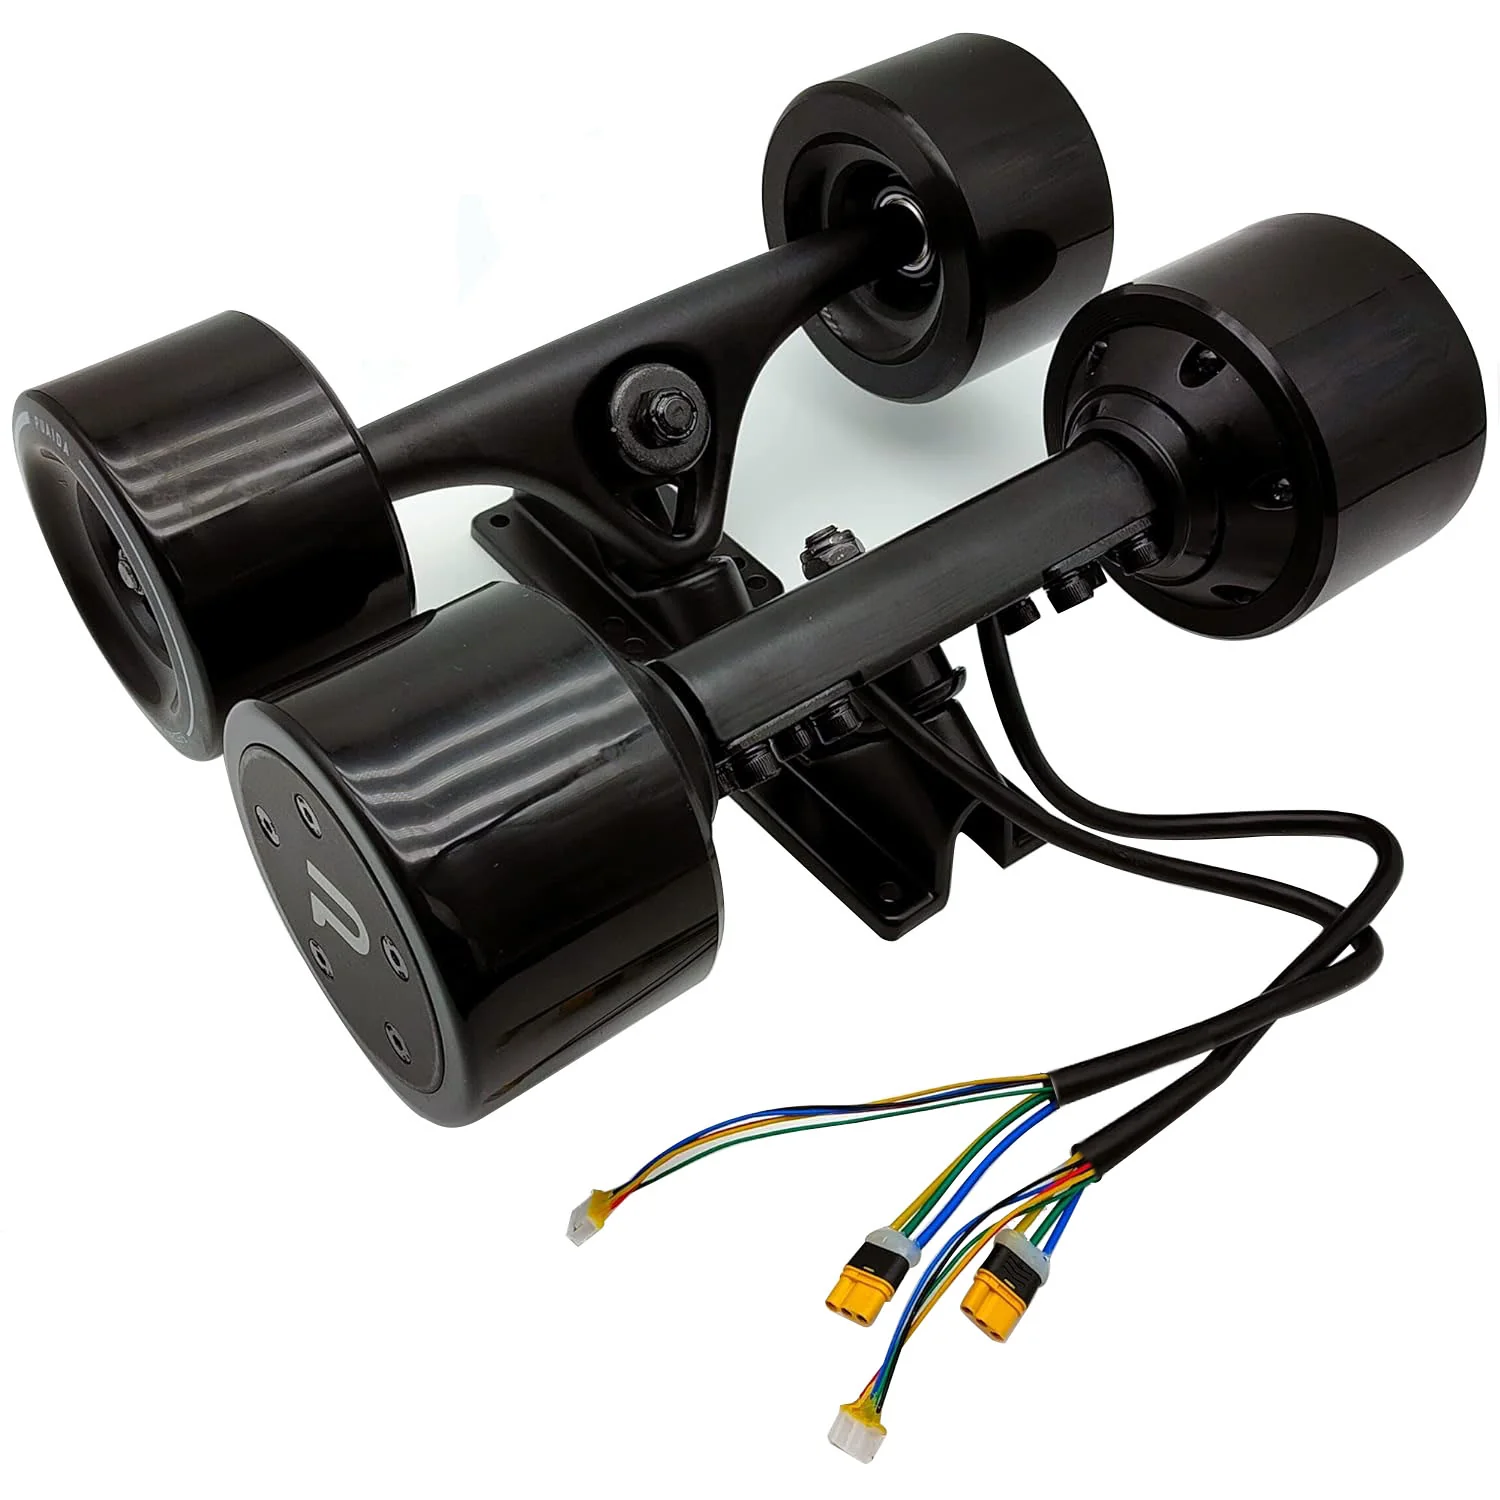
\includegraphics[height=8cm, width=1\linewidth, keepaspectratio]{obrazky-figures/drive-hub.png}
    \caption{Hub motor drive pohon\cite{Puaida}}\label{fig:hub-drive}
\end{figure*}

\newpage

\subsubsection{Direct drive}
Direct drive je spôsob pohonu, kedy sa motor nachádza na trucku a je priamo pripojený na koleso (\ref{fig:direct-drive}).
Tento spôsob je, podobne ako Hub motor drive, jednoduchší na údržbu.
Výmenu kolies je obmedzená len na kompatibilitu adaptéra, ktorý je potrebný pre pripojenie kolesa na motor, rovnako ako pri pohone pomocou remeňa.
Pri tomto spôsobe je možné dosiahnuť vyšší výkon a efektivitu, pretože nie je potrebné prenášať pohyb cez remeň alebo prevodovku.
Nevýhodou pri tomto spôsobe by mohla byť cena, ktorá je vyššia v~porovnaní s~ostatnými pohonmi.\cite{WikiElectricSkateboard}

\begin{figure*}[h]
    \centering
    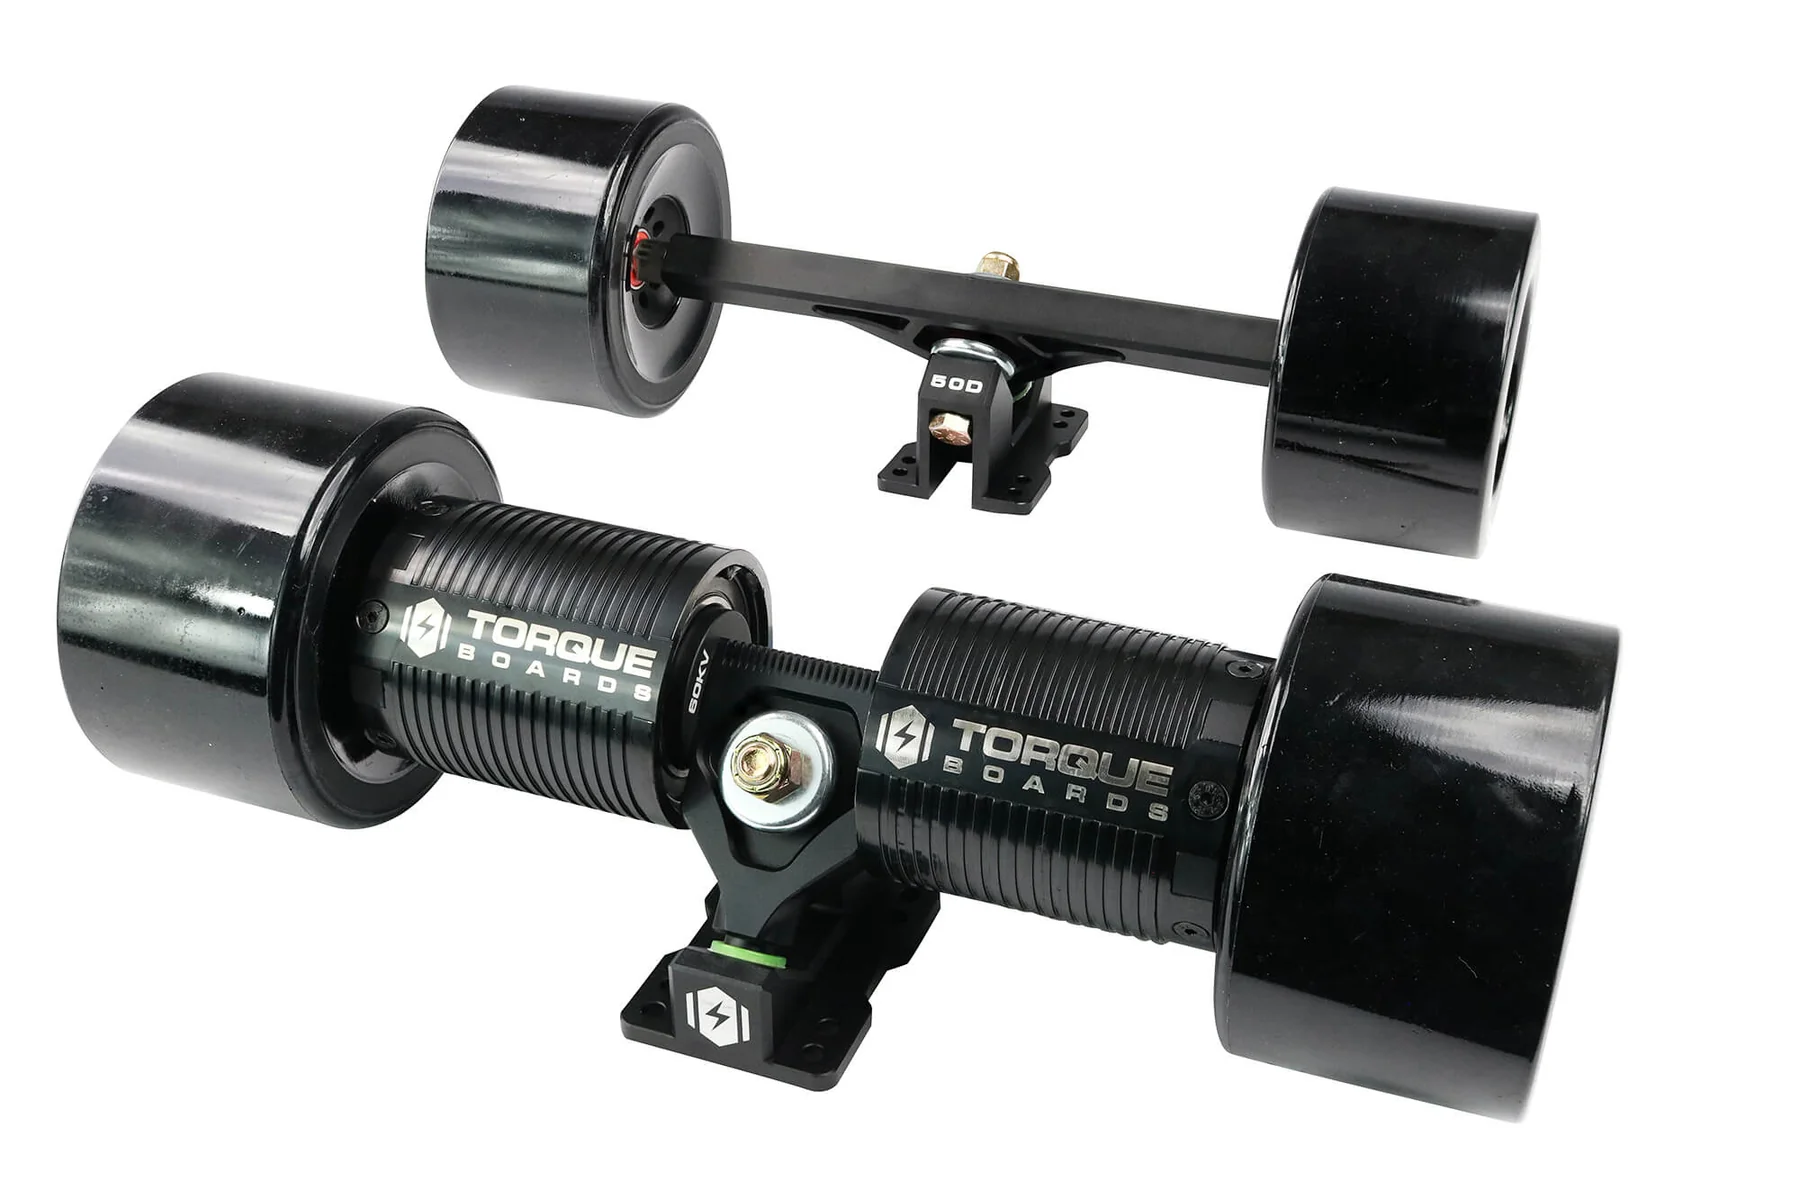
\includegraphics[height=7cm, width=1\linewidth, keepaspectratio]{obrazky-figures/drive-direct.png}
    \caption{Direct drive pohon\cite{TorqueBoards}}\label{fig:direct-drive}
\end{figure*}

\newpage

\subsection{ESC (Electronic Speed Controller)}
ESC (\ref{fig:esc}) je elektronický obvod, ktorý riadi a reguluje rýchlosť elektromotora.
V~modelárstve sa často používa na ovládanie BLDC motorov v~dronoch, RC autách a iných zariadeniach. 
ESC funguje ako sprostredkovateľ medzi batériou a motorom, pričom príjma PWM signál alebo signál z~iného podporovaného druhu komunikácie, ktorý následne podľa hodnoty mení frekvenckiu, dobu a spôsob spínania obvodu s~výkonovými tranzistormi.
Motor vďaka tomuto obvodu môže pracovať v~rôznych režimoch, ako napríklad jazda vpred, vzad, brzdenie alebo aj regeneratívne brzdenie, kedy motor funguje ako generátor a energia z~brzdenia sa vracia späť do akumulátora.\cite{Lauren}

\begin{figure*}[h]
    \centering
    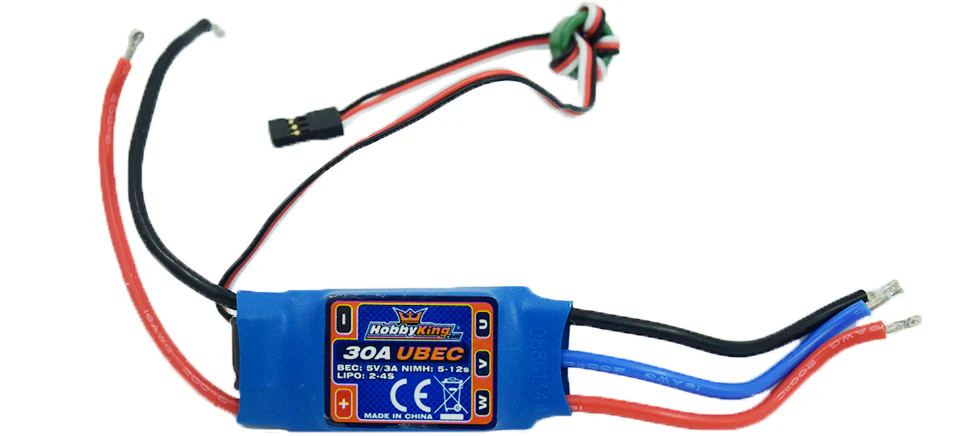
\includegraphics[height=6cm]{obrazky-figures/esc.png}
    \caption{Modelárske ESC\cite{Lauren}}\label{fig:esc}
\end{figure*}

\subsubsection{VESC (Vedder's Electronic Speed Controller)}
VESC (\ref{fig:vesc}) je špeciálny typ ESC, ktorý bol vyvinutý Benjaminom Vedderom pre modelárov a elektromobilistov.
Je dostupný ako open source projekt na platforme GitHub, kde je možné nájsť zdrojový kód, návody a aj možnosť prispievať k~jeho vývoju.
Jeho hlavnou výhodou oproti klasickému ESC je možnosť konfigurácie a kalibrácie všetkých parametrov, od ktorých závisí výkon a správanie ESC a motora.
VESC je možné pripojiť k~počítaču cez USB alebo Bluetooth a pomocou konfiguračného softvéru VESC Tool nastaviť jeho parametre.
Tieto parametre môžu byť napríklad maximálny prúd, hranice vstupného napätia akumulátora, maximálna rýchlosť a mnoho ďalších, ktoré konkrétny model ESC podporuje.
Okrem toho je možné sledovať v~reálnom čase dáta z~VESC o~napätí, prúde, stave a ovládaní motora.
VESC je tak ideálnym riešením pre elektromobilistov, ktorí chcú mať kontrolu nad svojím zariadením a zároveň mať možnosť meniť jeho parametre podľa svojich potrieb.\cite{VESC}

\begin{figure*}[h]
    \centering
    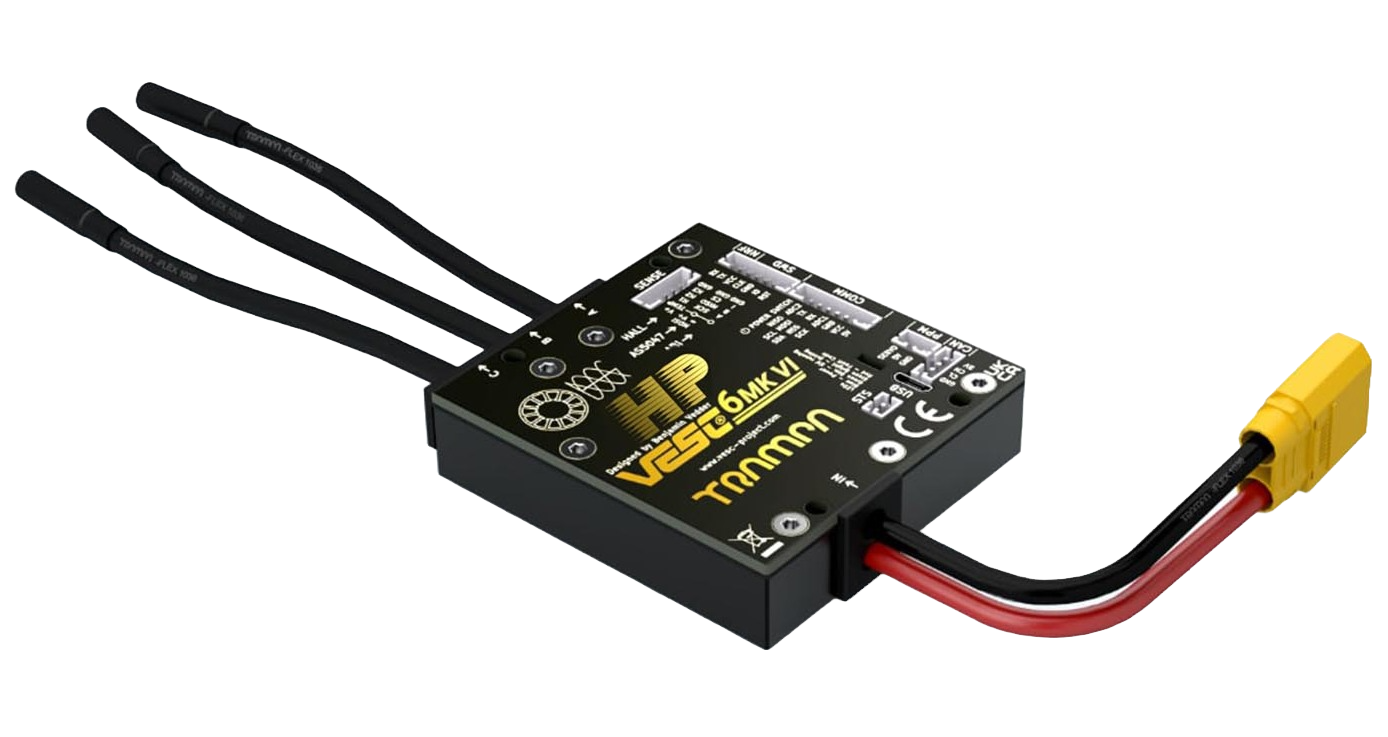
\includegraphics[height=8cm]{obrazky-figures/vesc.png}
    \caption{Programovatelné ESC --- VESC 6 MK6\cite{VESC}}\label{fig:vesc}
\end{figure*}

\section{Napájanie}
Napájanie je jedna ďaľšia z~dôležitejších častí elektronického zariadenia, pretože bez neho zariadenie nie je schopné fungovať.
Vzhľadom na to, že longboard s~elektrickým pohonom je prenosné zariadenie, je nutné zvoliť prenosný zdroj napájania, ktorý je ľahký, kompaktný a zároveň poskytuje dostatočný výkon pre pohon motora.

\subsection{Akumulátor}
Akumulátor alebo nabíjateľná batéria je dnes dôležitou súčasťou každého prenosného a znovupoužiteľného zariadenia od mobilných telefónov až po elektrické autá.
Oproti klasickým batériám umožňuje opakované nabíjanie a vybíjanie, čo znižuje celkové náklady na energiu a šetrí životné prostredie.\cite{Larminie}

Typicky sa akumulátor skladá z~viacerých článkov, ktoré sú pripojené sériovo alebo paralelne, aby sa dosiahli požadované vlastnosti.
Toto zapojenie sa vyjadruje pomocou násobku napätia a kapacity jedného článku, napríklad 10S2P znamená, že akumulátor je zložený zo 10 článkov v~sérii a 2 paralelne.
Z~aktuálne najpoužívanejších typov akumulátorových článkov sú najvhodnejšie Li-Ion (Lithium-Ion) a Li-Po (Lithium-Polymer) (\ref{fig:battery}).
Ich vlastnosti sú typické pre aplikácie, kde je potrebné dosiahnuť vysoký výkon a kapacitu pri relatívne nízkej hmotnosti a veľkosti.
Hustota energie týchto člankov sa pohybuje v~rozmedzí 100--250 Wh/kg.\cite{Itani}\cite{Robocraze}

\begin{figure*}[h]
    \centering
    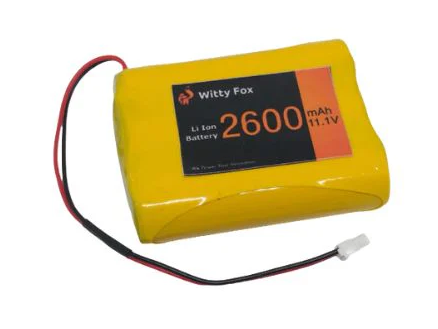
\includegraphics[width=0.48\linewidth]{obrazky-figures/li-ion.png}\hfill
    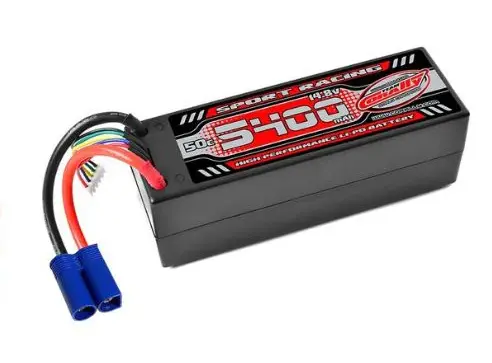
\includegraphics[width=0.48\linewidth]{obrazky-figures/li-po.png}
    \caption{Li-Ion a Li-Po akumulátory zložené z~viacerých článkov\cite{Robocraze}}\label{fig:battery}
\end{figure*}

Životnosť akumulátora, teda počet nabíjacích cyklov a kapacita, závisí od používania a správnej údržby.
Pre maximalizovanie životnosti je vhodné akumulátor udržiavať v~určitom rozsahu napätia, u~spomínaných článkov je to približne od 3V do 4,2V.
Hodnoty mimo tohto rozsahu môžu spôsobiť postupné zníženie kapacity alebo aj poškodenie a výbuch akumulátora.
Rovnako to platí aj pre teplotu, ktorá by nemala prekročiť 70°C a mala by byť udržiavaná v~rozmedzí 0--50°C.
Maximálne hodnoty prúdu sú obvykle udávané výrobcom, ale pre bezpečnosť a životnosť akumulátora je ideálne neprekračovať 1C*Ah (jeden násobok kapacity akumulátora).
Výrazne odporúčané je použiť ochranný obvod, ktorý monitoruje a reguluje tieto hodnoty a chráni akumulátor pred poškodením.\cite{BatterySpace}

\subsection{BMS (Battery Management System)}
BMS (\ref{fig:bms}) je zariadenie, ktoré monitoruje a riadi parametre akumulátora, ako napríklad napätie, prúd alebo teplotu.
Nachádza sa takmer vo všetkých moderných akumulátoroch a je nevyhnutnou súčasťou pre bezpečné používanie.
Jeho hlavnou úlohou je chrániť akumulátor pred prebitím, podbitím, preťažením, prehriatím, skratom alebo pred príliš vysokou teplotou.
V~prípade, ak by sa akýkoľvek z~týchto stavov vyskytol, BMS zvyčajne preruší prívod prúdu do alebo z~akumulátora a zabráni jeho poškodeniu.
BMS tak tvorí vrstvu ochrany medzi akumulátorom a zvyškom zariadenia.

Ďaľšou úlohou BMS môže byť aj balansovanie článkov, čo znamená, že sa stará o~to, aby boli všetky články nabíjané a vybíjané rovnomerne.
Táto funkcionalita sa avšak nevyskytuje u~všetkých BMS a je zvyčajne dostupná len u~drahších a rozmerovo väčších modelov.\cite{Bergveld}

\begin{figure*}[h]
    \centering
    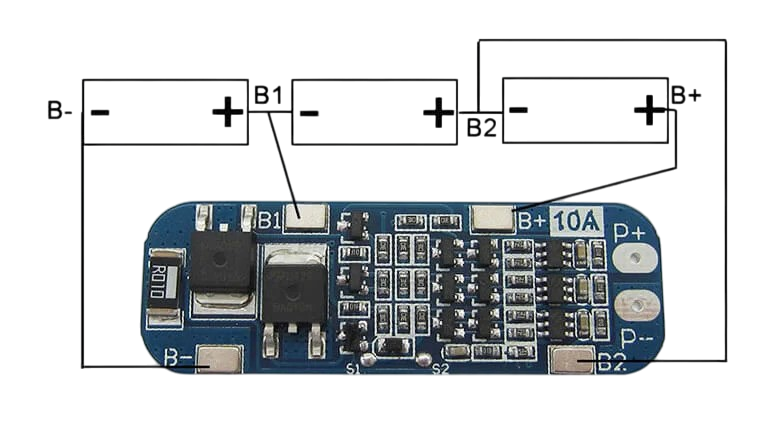
\includegraphics[height=6cm]{obrazky-figures/bms.png}
    \caption{Jednoduché BMS pre 3S akumulátor\cite{CampusComponent}}\label{fig:bms}
\end{figure*}

\section{Ovládanie a monitorovanie}
Longboard s~elektrickým pohonom vyžaduje sofistikovaný systém na zber, spracovanie a interpretáciu dát, ktorý zaisťuje bezpečné a efektívne ovládanie. 
Ovládanie je zvyčajne realizované pomocou bezdrôtového ovládača, ktorý komunikuje s~mikrokontrolérom v~longboarde cez bezdrôtové komunikačné rozhranie, ako je napríklad Bluetooth alebo 2,4 GHz RF.
Monitorovanie je zabezpečené pomocou senzorov, ktoré zbierajú dáta o~stave longboardu, ako je napríklad rýchlosť, náklon, teplota alebo stav akumulátora.
Táto kapitola sa zameriava na popis hardvérových a softvérových riešení, konkrétne na mikrokontrolér a senzory, ktoré tvoria hlavné komponenty systému ovládania a monitorovania.

\subsection{Mikrokontrolér}
Mikrokontrolér je integrovaný obvod, ktorý kombinuje procesor, pamäť a periférne rozhrania do jedného zariadenia. 
Tento \uv{samostatný procesor} je navrhnutý na vloženie do elektronických zariadení, ktoré nie sú tradičnými počítačmi. 
Používa sa na pridanie \uv{inteligencie} do rôznych elektronických aplikácií, pričom ponúka výhody nízkej ceny, jednoduchej implementácie a všestrannosti.

Na rozdiel od procesorov navrhnutých pre osobné počítače, mikrokontroléry obetujú extrémne vysoký výpočtový výkon výmenou za zabudovanú pamäť a periférie. 
Väčšina mikrokontrolérov zahŕňa na čipe statickú RAM na spracovanie údajov, nevolatilnú flash pamäť pre programový kód a často aj EEPROM pre uchovávanie konfigurácií či kalibračných dát. 
Tieto pamäte sú programovateľné a ich obsah ostáva zachovaný aj po výpadku napájania, čo je kľúčové pre aplikácie, kde sa vyžaduje trvalé uchovanie programového kódu.

Mikrokontroléry obsahujú aj rôzne integrované periférie, ktoré zjednodušujú ich použitie. 
Patria sem komunikačné rozhrania, ako napríklad SPI, I2C, USB, Ethernet alebo Bluetooth, analógové rozhrania na spracovanie signálov z~ADC, DAC alebo senzorov, a špecializované rozhrania, ako sú PWM, ovládače displejov alebo GPS. 
Tieto integrované periférie umožňujú eliminovať potrebu zložitého prepojenia viacerých externých komponentov.

Programovanie mikrokontroléra je proces, ktorý zahŕňa vytvorenie programu, ktorý riadi jeho správanie.
Vykonáva sa pomocou vývojového prostredia, ktoré umožňuje písanie, kompiláciu a nahrávanie programu do mikrokontroléra.
Vývojové prostredie (IDE) obsahuje nástroje na vytváranie programov v~jazykoch C alebo C++, ktoré sú najčastejšie používané pri programovaní mikrokontrolérov.
Po naprogramovaní je možné program nahrať do mikrokontroléra pomocou programátoru, ktorý je pripojený k~mikrokontroléru cez ICSP (In-Circuit Serial Programming) typicky pomocou UART, SPI alebo JTAG rozhrania.
Vývojové prostredie umožňuje aj ladenie programu, vďaka čomu je možné sledovať a meniť hodnoty premenných, ale aj kontrolovať stav registrov a chod programu.
Program sa typicky skladá z~viacerých častí, ktoré sú zvyčajne rozdelené do funkcií, ktoré vykonávajú konkrétne úlohy.
Tieto funkcie sú následne volané z~hlavného programu, ktorý riadi celkový chod programu.
Pri populárnych vývojových kitoch, ako sú Arduino alebo Teensy, je možné využiť knižnice, ktoré obsahujú hotové funkcie na prácu s~periférnymi zariadeniami, ako sú senzory, displeje alebo komunikačné rozhrania.

Dôležitou vlastnosťou mikrokontrolérov je možnosť ich programovania priamo v~zapojení.
To umožňuje jednoduchú aktualizáciu softvéru bez potreby vyberania zariadenia z~obvodu.
Jednoduchosť a všestrannosť robia mikrokontrolér, pri použití vývojových kitov, ideálnym na rýchly vývoj a testovanie systémov.\cite{Horowitz}

\subsection{Komunikáčné protokoly a rozhrania}
Na komunikáciu s~periférnymi zariadeniami a užívateľom je potrebné mať k~dispozícii rôzne komunikačné protokoly a rozhrania.
Umožňujú prenos dát medzi mikrokontrolérom a inými zariadeniami, ako sú senzory, displeje, mikrokontroléry a počítače.

\subsubsection{WiFi a Bluetooth}
WiFi technológia umožňuje mikrokontrolérom komunikovať s~internetom alebo lokálnou sieťou na vzdialenosť niekoľkých desiatok metrov. 
Vďaka vysokej prenosovej rýchlosti je ideálna na aplikácie vyžadujúce veľký objem dát.

Bluetooth je technológia na krátke vzdialenosti, ktorá sa využíva na priamu komunikáciu medzi zariadeniami. 
Napriek nižšej prenosovej rýchlosti je vhodná pre aplikácie, kde je dôležitá nízka spotreba energie a jednoduché spárovanie zariadení.\cite{Afaneh}

\subsubsection{UART, SPI a I2C}
Komunikačné protokoly sú dôležitou súčasťou vstavaných systémov, pretože umožňujú prenos dát medzi mikrokontrolérom a periférnymi zariadeniami.

UART (Universal Asynchronous Receiver-Transmitter) je jednoduché sériové komunikačné rozhranie na prenos dát medzi dvoma zariadeniami. 
Je známe svojou jednoduchosťou a širokým použitím, napríklad na debugovanie a konfiguráciu.
SPI (Serial Peripheral Interface) je vysokorýchlostný protokol využívaný na komunikáciu s~perifériami, ako sú senzory, displeje alebo pamäťové moduly.
Ponúka flexibilitu a rýchlosť, no vyžaduje viac pinov na prepojenie.
I2C (Inter-Integrated Circuit) je ďalší populárny protokol, ktorý umožňuje komunikáciu medzi viacerými zariadeniami po dvoch linkách, čím šetrí piny.
Je ideálny pre aplikácie s~veľkým množstvom senzorov.\cite{Horowitz}

\subsubsection{ADC, DAC a PWM}
Na pripojenie analógových a digitálnych zariadení je potrebné mať k~dispozícii periférne rozhrania, ktoré umožňujú spracovanie týchto signálov.

ADC (Analog-to-Digital Converter) premieňa analógové signály na digitálne hodnoty, ktoré môžu byť spracované mikrokontrolérom. 
To je užitočné pri práci so senzormi merajúcimi fyzikálne veličiny, ako je napríklad teplota. 
DAC (Digital-to-Analog Converter) vykonáva opačný proces, teda premieňa digitálne hodnoty na analógové signály, ktoré sa môžu využiť na riadenie analógových zariadení, ako sú reproduktory alebo motory. 
PWM (Pulse Width Modulation) je technika generovania digitálnych signálov, ktoré simulujú analógové výstupy. 
Používa sa na reguláciu intenzity svetla LED, rýchlosti motorov alebo riadenie výkonových zariadení.\cite{Horowitz}

\subsection{Senzory}
Senzory zohrávajú kľúčovú rolu vo vstavaných systémoch, pretože umožňujú zber dát o~okolitom prostredí a stave zariadenia.
Každý senzor je navrhnutý na zber konkrétneho typu dát, ktoré sú následne spracované mikrokontrolérom.
V~tejto práci boli zahrnuté nasledujúce senzory.

\subsubsection{Hall senzor}
Hall senzor je zariadenie, ktoré slúži na meranie magnetického poľa.
Využíva princíp Hallovho efektu, kedy sa v~prítomnosti magnetického poľa generuje elektrické napätie.
Tento senzor je často používaný na detekciu polohy, rýchlosti alebo rotácie.
Používa na detekciu otáčok motora, ktoré sú následne spracované mikrokontrolérom na reguláciu rýchlosti alebo smeru jazdy.
Okrem toho je možné využiť Hall senzor na detekciu pozície pri pedáloch alebo spínačoch.\cite{Soltero}

\subsubsection{Akcelerometer}
Akcelerometer slúži na meranie zrýchlenia, typicky v~troch osiach.
Umožňuje sledovať pohyb zariadenia, vrátane otrasov a vibrácií.
Akcelerometer vyhodnocuje aj gravitačné zrýchlenie a umožňuje tak zistiť náklon zariadenia.\cite{Adafruit}

\subsubsection{Gyroskop}
Gyroskop dopĺňa akcelerometer o~možnosť merania uhlového zrýchlenia v~troch osiach.
Poskytuje informácie o~zmene orientácie alebo rotácie zariadenia.
Slúži na presnejšie sledovanie pohybu a detekciu náklonu.\cite{Adafruit}

\subsubsection{Magnetometer}
Magnetometer meria magnetické pole okolia a umožňuje určiť orientáciu zariadenia vo vzťahu k~zemskému magnetickému polu.
Táto informácie je vhodná pre zaznamenávanie orientácie a navigáciu.\cite{Adafruit}

\subsubsection{Teplotný senzor}
Teplotný senzor je súčiastka alebo zariadenie určené na meranie teploty prostredia, povrchu alebo látky.
Existuje viacero druho teplotných senzorov. Najčastejšie používanými sú termistory, ktoré menia svoj odpor v~závislosti od teploty.
Teplotný senzor môže pomôcť zvýšiť bezpečnosť zariadenia.\cite{IQS}

\chapter{Analýza trhu}\label{analyza_trhu}

Na trhu existuje množstvo dostupných riešení pre vývoj longboardov s~elektrickým pohonom, ktoré sa líšia výkonom, cenou, dizajnom a funkcionalitou.
Každý výrobca sa snaží vytvoriť zariadenie, ktoré by spĺňalo požiadavky zákazníka a bolo konkurencieschopné.
V~tejto kapitole sú zhrnuté aj niektoré z~aktuálne najpopulárnejších riešení dostupných na trhu ale aj niektoré zaujímavé koncepty, ktoré môžu slúžiť ako inšpirácia pre vývoj vlastného zariadenia.\cite{Gell}
Medzi porovnaniami sa nenechádzajú všetky dostupné modely, ako napríklad off-road longboardy, ale len tie, ktoré sú relevantné pre túto prácu a prinášajú rôzny prístup k~vývoju a dizajnu.

\newpage

\section{Boosted}
Boosted je bývalý americký výrobca elektrických longboardov a kolobežiek.
Ich longboardy boli jednými z~prvých na trhu a patrili medzi najpopulárnejšie, avšak ich výroba a vývoj boli ukončené.
Ponúkali kvalitné a výkonné longboardy, ktoré boli dostupné s~pohonom pomocou remeňa na dvoch kolesách a vymeniťelným Li-Ion akumulátorom.
Dojazd dosky tak mohol byť predĺžený jednoduchou výmenou akumulátora.
Nevýhodou longboardov bola cena, ktorá vzhadom na ich popularitu a kvalitu bola vyššia ako u~iných výrobcov.\cite{Boosted} 

\begin{table}[h]
    \centering
    \begin{tabular}{|l|l|}
        \hline
        \textbf{Parameter} & \textbf{Hodnota} \\ \hline
        Maximálna rýchlosť & 38 km/h \\ \hline
        Dojazd & 22 km \\ \hline
        Maximálne stúpanie & 25\% \\ \hline
        Počet jazdných režimov & 5 \\ \hline
        Akumulátor & Li-Ion 199 Wh \\ \hline
        Typ akumulátorového článku & \it{neuvedený} \\ \hline
        Doba nabíjania & 1 h 45 min \\ \hline
        Výkon motora & 2x 1050 W \\ \hline
        Typ pohonu & Belt drive \\ \hline
        Hmotnosť dosky & 7,7 kg \\ \hline
        Cena & \$1599 ($\approx$1550 €) \\ \hline
    \end{tabular}
    \caption{Parametre elektrického longboardu Boosted Board Stealth (Obrázok~\ref{fig:boosted})~\cite{Boosted}}\label{tab:boosted}
\end{table}

Ovládanie longboardu pomocou bezdrôtového ovládača je priame a intuitívne.
V~hornej časti ovládača sa nachádza otočné kolečko, ktoré slúži na zrýchlenie a brzdenie.
Pre jazdu je potrebné stlačiť tlačidlo na vnútornej strane ovládača, inak sa motor nezapne.
Ak sa tlačidlo uvoľní počas jazdy, longboard začne brzdiť.
Na ovládači je tiež možné sledovať stav batérie dosky a ovládača, vďaka multifunkčnému tlačidlu v~spodnej časti, ktoré tiež umožňuje ovládač zapnúť/vypnúť a prepínať jazdné režimy.\cite{BoostedManual}

\begin{figure*}[h]
    \centering
    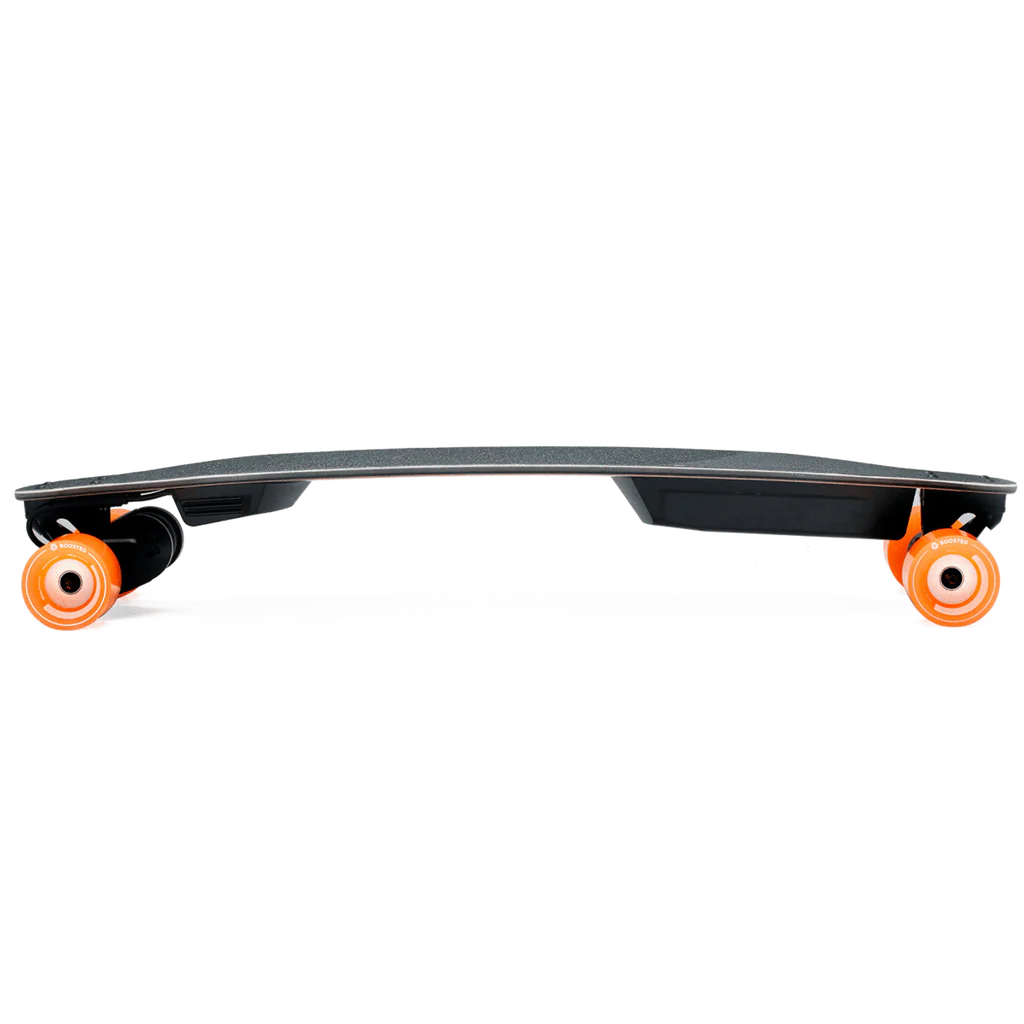
\includegraphics[width=0.48\linewidth]{obrazky-figures/brand-reviews/boosted-longboard.png}\hfill
    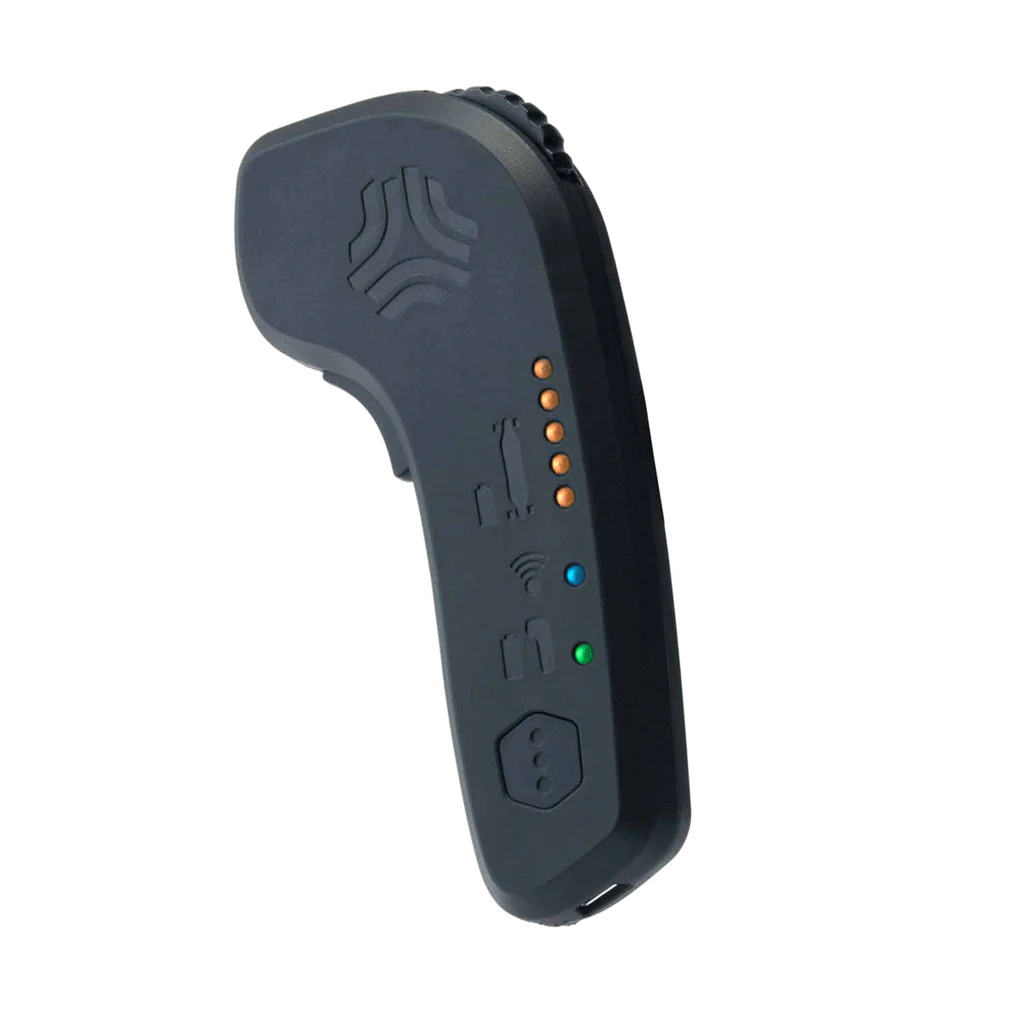
\includegraphics[width=0.48\linewidth]{obrazky-figures/brand-reviews/boosted-controller.png}
    \caption{Boosted Board Stealth longboard a ovládač\cite{BoostedGuys}}\label{fig:boosted}
\end{figure*}

Aplikácia Boosted bola dostupná pre mobilné zariadenia s~operačným systémom iOS a Android.
Pomocou aplikácie bolo možné monitorovať stav batérie, rýchlosť, prejdenú vzdialenosť alebo aj trasu jazdy na mape.
Umožňovala tiež nastaviť jazdné režimy, konfigurovať nastavenia a aktualizovať firmvér dosky a ovládača.\cite{BoostedApp}

\section{Evolve}
Evolve je austrálsky výrobca elektrických longboardov a kolobežiek, ktorý ponúka širokú škálu modelov prispôsobené rôznym štýlom jazdy, od mestských až po terénne.
Zaujímavým prvkom je modularita –-- možnosť výmeny kolies a prispôsobenia dosky podľa preferencií. 
Výhodou Evolve je dlhý dojazd, stabilita pri vyšších rýchlostiach a pohodlné ovládanie.
Nevýhodou môže byť vyššia cena a hmotnosť dosiek, čo môže znepríjemniť prenášanie. 
Modulárny dizajn tiež vyžaduje určitú technickú zručnosť, najmä pri údržbe a výmene dielov.
Evolve ponúka lepšiu kvalitu a flexibilitu ako jeho konkurencia, no za cenu vyššej investície.

\begin{table}[h]
    \centering
    \begin{tabular}{|l|l|}
        \hline
        \textbf{Parameter} & \textbf{Hodnota} \\ \hline
        Maximálna rýchlosť & 44 km/h \\ \hline
        Dojazd & 50 km \\ \hline
        Maximálne stúpanie & 30 \% \\ \hline
        Počet jazdných režimov & 4 \\ \hline
        Akumulátor & Li-Ion 504 Wh, 10S4P \\ \hline
        Typ akumulátorového článku & Samsung 18650 35E, 3500 mAh \\ \hline
        Doba nabíjania & 4--5 h \\ \hline
        Výkon motora & 2x 3000 W \\ \hline
        Typ pohonu & Belt drive \\ \hline
        Hmotnosť dosky & 11.1 kg \\ \hline
        Cena & \$1199 ($\approx$1160 €) \\ \hline
    \end{tabular}
    \caption{Parametre elektrického longboardu Evolve GTR Bamboo Street (Obrázok~\ref{fig:evolve})~\cite{Evolve}}\label{tab:evolve}
\end{table}

Ovládač je odlišný od ostatných značiek.
Má ergonomický \uv{pištolový} tvar, ktorý umožňuje pohodlné držanie.
Zrýchlenie sa ovláda pomocou ukazováku na vnútornej časti ovládača, ktorý sa stlačí smerom k~dlani.
Brzdenie je možné pomocou palca, ktorý sa stlačí smerom vpred.
Poistka na spodnej strane ovládača umožňuje jazdu len po stlačení, čím sa minimalizuje riziko neúmyselného štartu.
Na ovládači je tiež možné sledovať stav ovládača a dosky pomocou LED dispeja v~hornej časti.
Ďaľšie tlačidlá umožňujú prepínanie v~menu na ovládanie jazdných režimov a osvetlenia alebo aj zobrazenie dát o~jazde.
Po určitom čase nečinnosti sa ovládač automaticky vypne, čím sa šetrí energia.
Ovládač je kompatibilný s~viacerými modelmi značky Evolve.

\begin{figure*}[h]
    \centering
    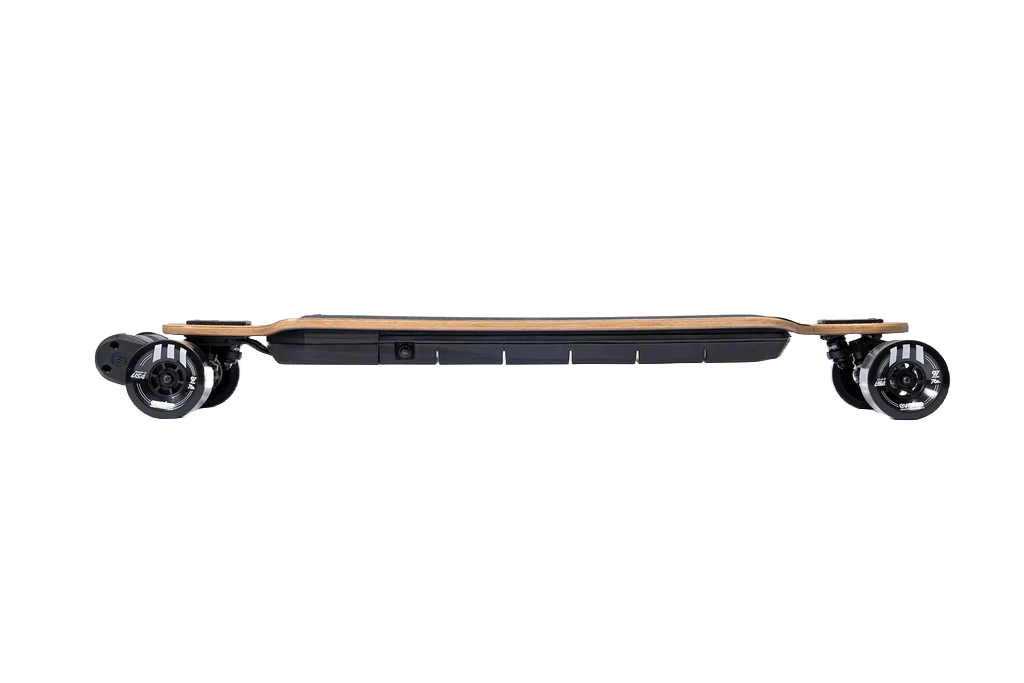
\includegraphics[width=0.48\linewidth]{obrazky-figures/brand-reviews/evolve-longboard.png}\hfill
    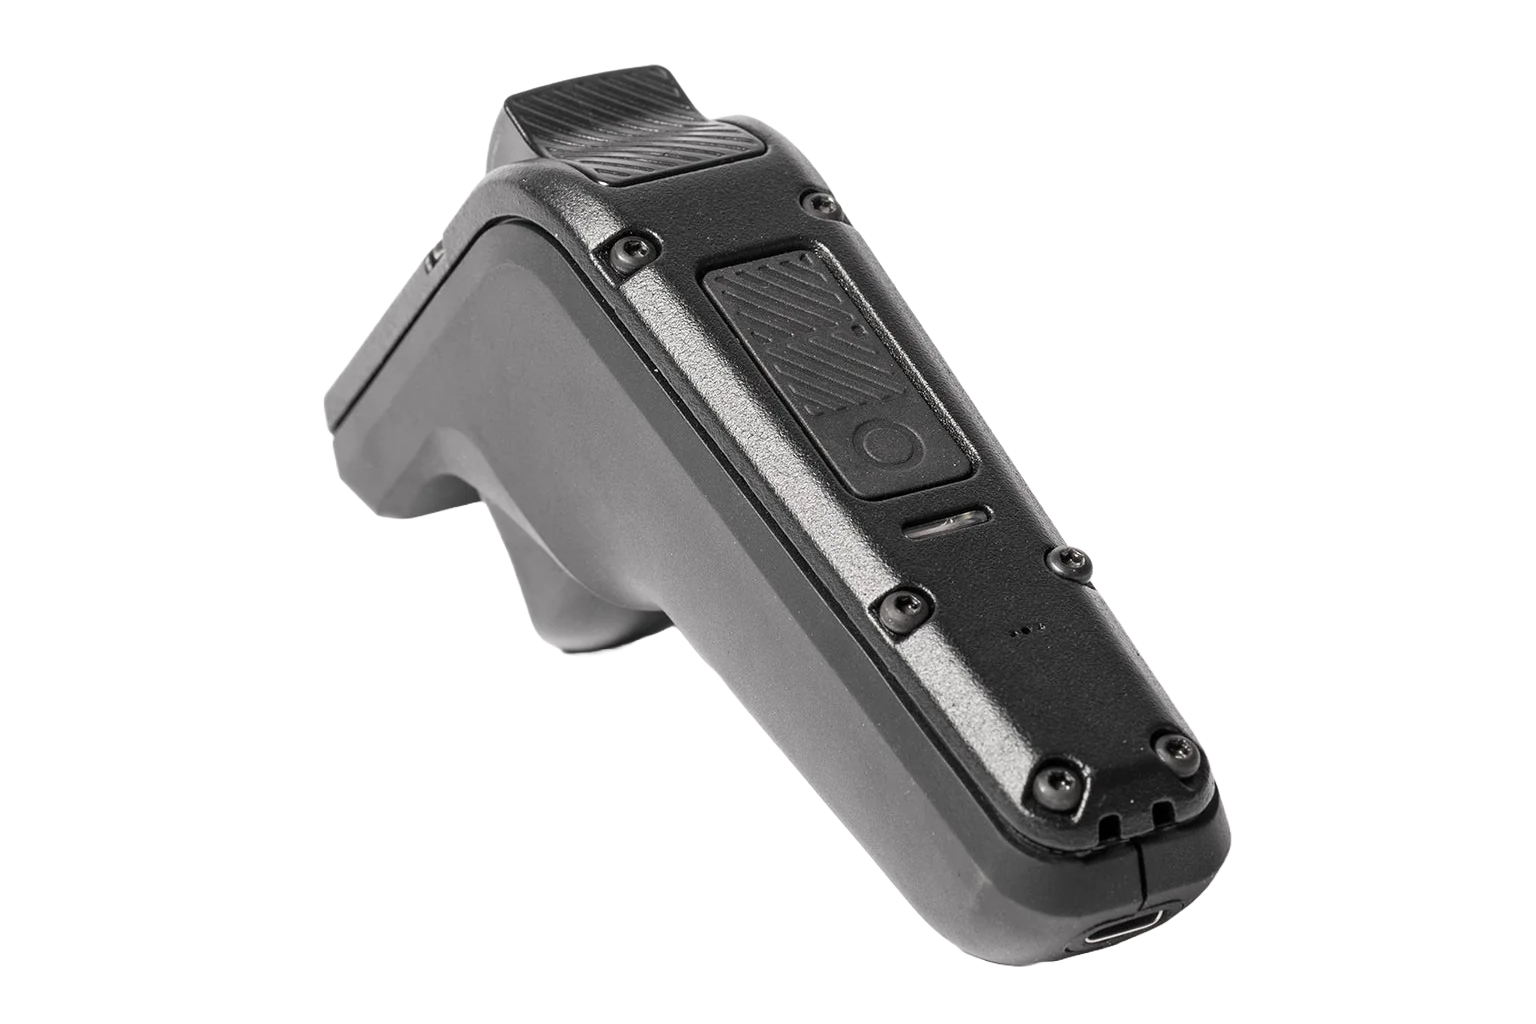
\includegraphics[width=0.48\linewidth]{obrazky-figures/brand-reviews/evolve-controller.png}
    \caption{Evolve GTR Bamboo Street longboard a ovládač\cite{Evolve}}\label{fig:evolve}
\end{figure*}

Aplikácia Evolve je dostupná pre mobilné zariadenia s~operačným systémom iOS a Android.
Pomocou aplikácie je možné konfigurovať a vytvoriť jazdné režimy a jednotlivé parametre jazdy, ako intenzitu brzdenia a akcelerácie.
Umožňuje sledovať stav batérie, teplotu komponentov, prejdenú vzdialenosť.
V~aplikácii je tiež možné nahrávať trasu jazdy na mape a zdieľať ju s~ostatnými.
Okrem užívatelsky prívetivej konfigurácie umožňuje aplikácia aj aktualizáciu firmvéru dosky a ovládača.\cite{Evolve}

\section{Meepo}
Meepo je čínska značka známa svojimi cenovo dostupnými elektrickými skateboardmi, ktoré sú ideálne pre začiatočníkov. 
Dosky sú jednoduché na používanie a ponúkajú dobrý výkon za svoju cenu, pričom poskytujú slušný dojazd a zrýchlenie.
Meepo sa zameriava na praktickosť a spoľahlivosť, čo z~nej robí skvelú voľbu pre tých, ktorí chcú vyskúšať elektrický skateboard bez veľkých nákladov. 
Nevýhodou je nižšia kvalita materiálov a kratšia životnosť v~porovnaní s~prémiovými značkami. 
Taktiež nemajú taký elegantný dizajn ani modularitu ako niektoré konkurenčné značky. 
Meepo je však obľúbený pre svoju jednoduchú opravitelnosť a cenovú dostupnosť.

\begin{table}[h]
    \centering
    \begin{tabular}{|l|l|}
        \hline
        \textbf{Parameter} & \textbf{Hodnota} \\ \hline
        Maximálna rýchlosť & 45 km/h \\ \hline
        Dojazd & 32 km \\ \hline
        Maximálne stúpanie & 18\% \\ \hline
        Počet jazdných režimov & 4 \\ \hline
        Akumulátor & Li-Ion 288 Wh, 10S2P \\ \hline
        Typ akumulátorového článku & Samsung 21700 40T, 4000 mAh \\ \hline
        Doba nabíjania & 2 h 45 min \\ \hline
        Výkon motora & 2x 500 W \\ \hline
        Typ pohonu & Hub motor \\ \hline
        Hmotnosť dosky & 8.8 kg \\ \hline
        Cena & \$699 ($\approx$685 €) \\ \hline
    \end{tabular}
    \caption{Parametre elektrického longboardu Meepo V5 ER (Obrázok~\ref{fig:meepo})~\cite{Meepo}}\label{tab:meepo}
\end{table}

Ovládač Meepo longboardov má ergonomický dizajn s~otočným kolečkom na zrýchlenie a brzdenie.
Funkcia jazdy Cruise Control umožňuje udržiavať konštantnú rýchlosť bez nutnosti držať otočné kolečko.
Na ovládači sa nachádzajú aj tlačidlá na prepínanie jazdných režimov.
Možnosť sledovať stav dosky a ovládača je zabezpečená pomocou displeja na ovládači.
Ovládač je kompatibilný s~viacerými modelmi značky Meepo.

\begin{figure*}[h]
    \centering
    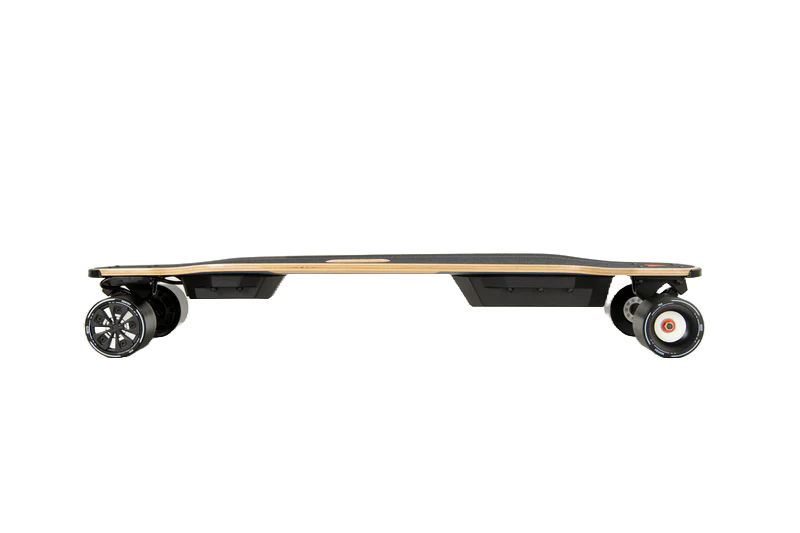
\includegraphics[width=0.48\linewidth]{obrazky-figures/brand-reviews/meepo-longboard.png}\hfill
    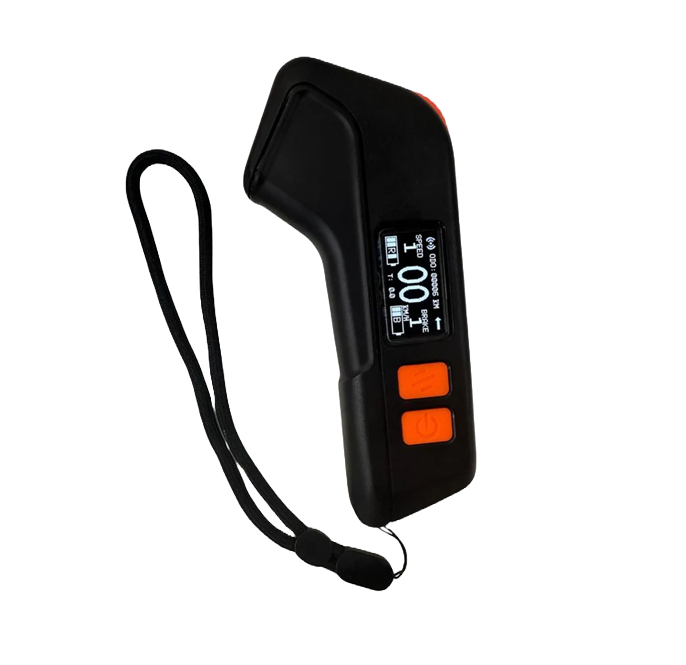
\includegraphics[width=0.48\linewidth]{obrazky-figures/brand-reviews/meepo-controller.png}
    \caption{Meepo V5 ER longboard a ovládač\cite{Meepo}}\label{fig:meepo}
\end{figure*}

Značka Meepo neponúka mobilnú aplikáciu pre sledovanie a konfiguráciu dosky.\cite{Meepo}

\section{WowGo}
WowGo je ďalší čínsky výrobca elektrických longboardov, ktorý sa snaží kombinovať kvalitu a dostupnosť, čím oslovujú široké spektrum jazdcov. 
Ich dosky sú známe plynulým zrýchlením, tichými motormi a komfortnou jazdou, vďaka čomu sú vhodné na mestské použitie aj dlhšie trasy. 
Dizajn je minimalistický, pričom kvalita spracovania je vyššia ako u~niektorých lacnejších značiek.
Podobne ako Meepo aj WowGo ponúka jednoduchú opravitelnosť a cenovú dostupnosť. 
Nevýhodou je o~niečo kratší dojazd a menej výkonné motory v~porovnaní s~drahšími značkami. 
Pre začiatočníkov a mierne pokročilých jazdcov je však WowGo vynikajúcou voľbou.

\begin{table}[h]
    \centering
    \begin{tabular}{|l|l|}
        \hline
        \textbf{Parameter} & \textbf{Hodnota} \\ \hline
        Maximálna rýchlosť & 45 km/h \\ \hline
        Dojazd & 33 km \\ \hline
        Maximálne stúpanie & 30\% \\ \hline
        Počet jazdných režimov & 4 \\ \hline
        Akumulátor & Li-Ion 345 Wh, 12S2P \\ \hline
        Typ akumulátorového článku & Samsung 21700 40T, 4000 mAh \\ \hline
        Doba nabíjania & 2 h 30 min \\ \hline
        Výkon motora & 2x 700 W \\ \hline
        Typ pohonu & Belt drive \\ \hline
        Hmotnosť dosky & 8.4 kg \\ \hline
        Cena & \$899 ($\approx$870 €) \\ \hline
    \end{tabular}
    \caption{Parametre elektrického longboardu WowGo Pioneer X4 (Obrázok~\ref{fig:wowgo})~\cite{WowGo}}\label{tab:wowgo}
\end{table}

Ovládanie WowGo longboardov je taktiež veľmi minimalistické.
Typické otočné kolečko na ovládači slúži na zrýchlenie a brzdenie.
Tlačidlo na strane slúži na ovládanie jazdných režimov, osvetlenia a displeja.

\begin{figure*}[h]
    \centering
    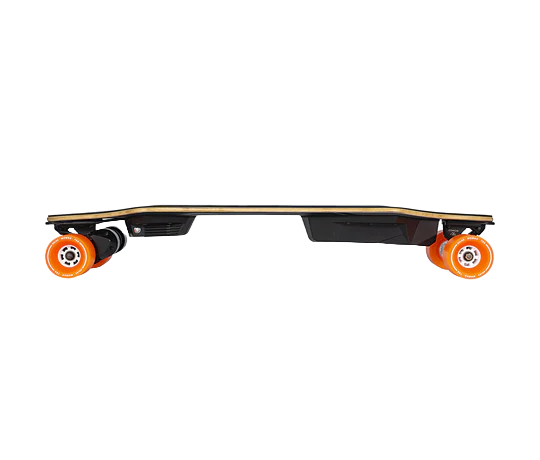
\includegraphics[width=0.48\linewidth]{obrazky-figures/brand-reviews/wowgo-longboard.png}\hfill
    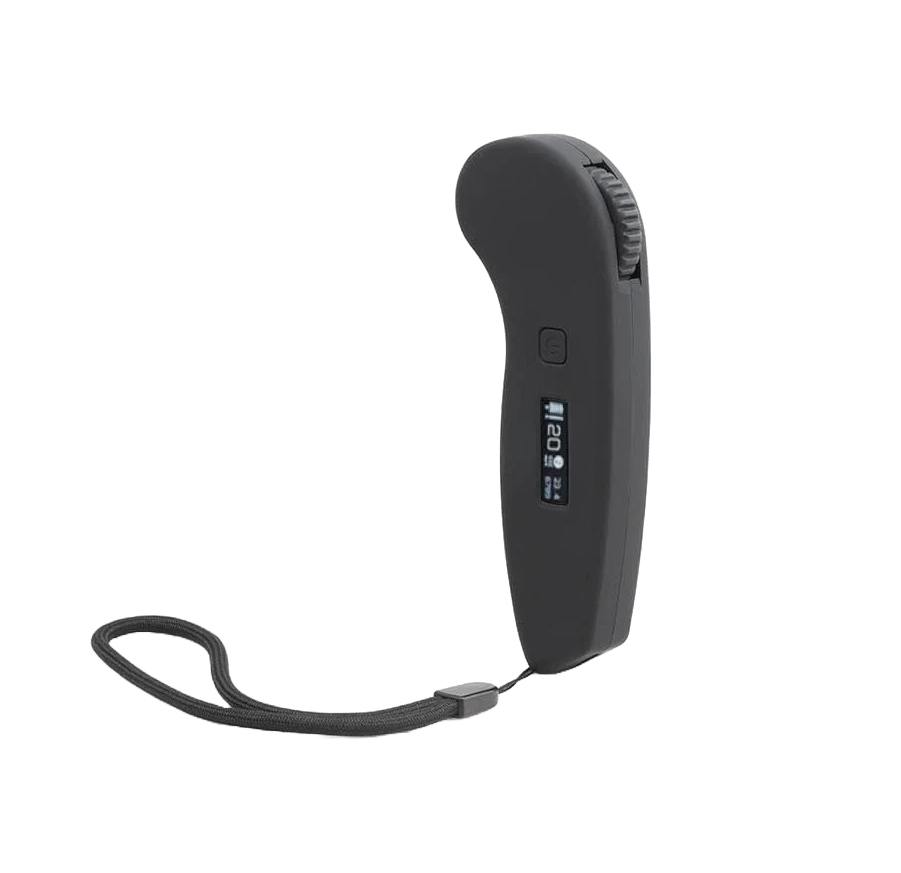
\includegraphics[width=0.48\linewidth]{obrazky-figures/brand-reviews/wowgo-controller.png}
    \caption{WowGo Pioneer X4 longboard a ovládač\cite{WowGo}}\label{fig:wowgo}
\end{figure*}

Aplikácia WowGo je dostupná pre mobilné zariadenia s~operačným systémom iOS a Android.
Pre spojenie s~doskou je potrebné mať zapnutý ovládač a dosku.
Aplikácia je všeobecnou platformou pre ovládanie a monitorovanie smart zariadení, takže nie je špecificky prispôsobená pre longboardy.\cite{WowGo}

\section{Torqueboards}
Torqueboards je americký výrobca elektrických longboardov a kolobežiek, ktorý sa zameriava na výkonné a robustné dosky pre náročných jazdcov.
Ich modely sú vybavené silnými motormi a kapacitnými batériami, čo zabezpečuje vysoký výkon a dojazd.
Torqueboards ponúka aj možnosť vlastného zostavenia dosky podľa preferencií zákazníka, čo je ideálne pre skúsených jazdcov, ktorí hľadajú špecifické vlastnosti.
Možnosť konfigurácie ESC je veľkou výhodou pre skúsených užívateľov.
Úprava jazdných vlastností a nastavení umožňuje s~doskou experimentovať a prispôsobiť aj na ovládanie pomocou iného zariadenia ako je ovládač. 
Nevýhodou značky je vyššia cena a hmotnosť dosiek, ktoré môžu byť nepraktické pre začiatočníkov, ktorí preferujú ľahšie a lacnejšie zariadenia.\cite{TorqueBoards}

\begin{table}[h]
    \centering
    \begin{tabular}{|l|l|}
        \hline
        \textbf{Parameter} & \textbf{Hodnota} \\ \hline
        Maximálna rýchlosť & 65 km/h \\ \hline
        Dojazd & 48 km \\ \hline
        Maximálne stúpanie & 30\% \\ \hline
        Počet jazdných režimov & 4 \\ \hline
        Akumulátor & Li-Ion 432 Wh, 12S4P \\ \hline
        Typ akumulátorového článku & Molicel 21700 P42A, 4200 mAh \\ \hline
        Doba nabíjania & 2 h 30 min \\ \hline
        Výkon motora & 2x 4500 W \\ \hline
        Typ pohonu & Belt drive \\ \hline
        Hmotnosť dosky & 9.5 kg \\ \hline
        Cena & \$1499 ($\approx$1480 €) \\ \hline
    \end{tabular}
    \caption{Parametre elektrického longboardu TorqueBoards Street (Obrázok~\ref{fig:torqueboards})~\cite{TorqueBoards}}\label{tab:torqueboards}
\end{table}

Na ovládanie Torqueboards longboardov je možné použiť akýkoľvek ovládač s~kompatibilným protokolom, čo umožňuje využiť aj vlastné riešenia.
Značka ponúka aj ovládače, ktoré sa veľmi podobajú na ovládače iných značiek.
Na riadenie používajú otočné kolečko a niekoľko multifunkčných tlačidiel.
Zobrazenie stavu batérie longboardu na ovládači je možné len pomocou indikátorov a vyžadujuje pripojenie vysielaču ku kontaktom akumulátora. 

\begin{figure*}[h]
    \centering
    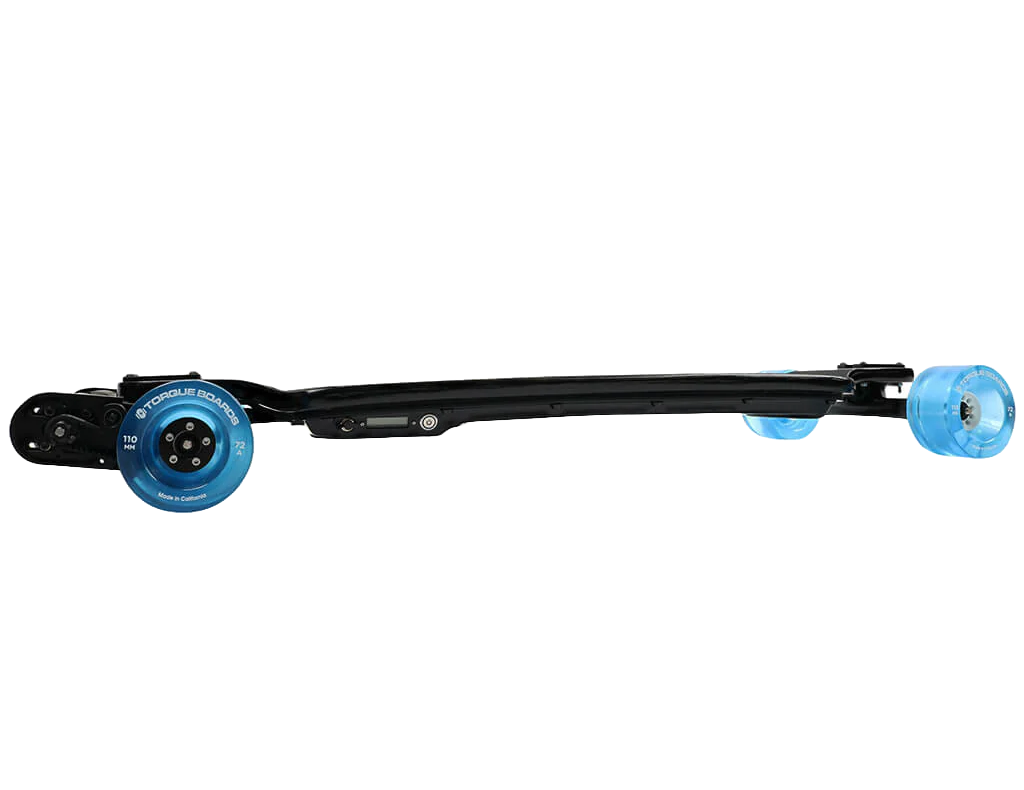
\includegraphics[width=0.48\linewidth]{obrazky-figures/brand-reviews/torque-longboard.png}\hfill
    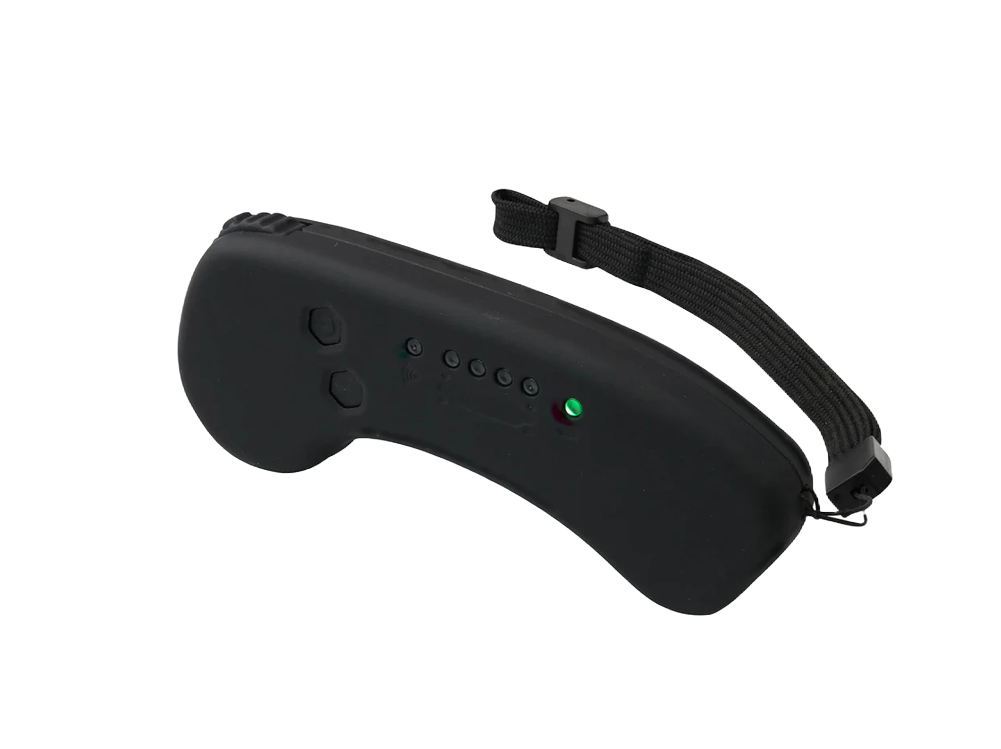
\includegraphics[width=0.48\linewidth]{obrazky-figures/brand-reviews/torque-controller.png}
    \caption{TorqueBoards Street longboard a ovládač\cite{TorqueBoards}}\label{fig:torqueboards}
\end{figure*}

TorqueBoards neponúka vlastnú aplikáciu na sledovanie a konfiguráciu dosky, ale umožňuje používať aplikácie tretích strán, ktoré sú schopné komunikovať s~ESC.
Na používanie týchto aplikácií je potrebné mať k~ESC pripojený komunikáčný modul a konfigurovať ESC na komunikáciu s~aplikáciou.\cite{TorqueBoards}

\section{Backfire}
Backfire je americký výrobca elektrických longboardov, ktorý sa zameriava na kvalitu a výkon za prijateľnú cenu.
Ich dosky sú známe pre svoju spoľahlivosť, pohodlnú jazdu a jednoduché ovládanie.
Backfire ponúka širokú škálu modelov pre rôzne štýly jazdy, od mestských po terénne.
Výhodou je dobrý pomer cena/výkon, kvalitné materiály a dizajn.
Nevýhodou môže byť nižší výkon a dojazd v~porovnaní s~drahšími značkami.

\begin{table}[h]
    \centering
    \begin{tabular}{|l|l|}
        \hline
        \textbf{Parameter} & \textbf{Hodnota} \\ \hline
        Maximálna rýchlosť & 46 km/h \\ \hline
        Dojazd & 40 km \\ \hline
        Maximálne stúpanie & 30\% \\ \hline
        Počet jazdných režimov & 3 \\ \hline
        Akumulátor & Li-Ion 363 Wh, 14S2P \\ \hline
        Typ akumulátorového článku & 21700, 3600 mAh \\ \hline
        Doba nabíjania & 2 h 30 min \\ \hline
        Výkon motora & 2x 700 W \\ \hline
        Typ pohonu & Hub motor drive \\ \hline
        Hmotnosť dosky & 10 kg \\ \hline
        Cena & \$649 ($\approx$630 €) \\ \hline
    \end{tabular}
    \caption{Parametre elektrického longboardu Backfire G5 (Obrázok~\ref{fig:backfire})~\cite{Backfire}}\label{tab:backfire}
\end{table}

Ovládač Backfire využíva na zrýchlenie a brzdenie otočné kolečko na vrchnej strane ovládača.
Dizajn s~otvor na ukazovák umožňuje pohodlné držanie a ovládanie.
Na ovládači sa nachádza niekoľko tlačidiel na prepínanie jazdných režimov a prepínač na zmenu smeru jazdy. 
Na informovanie užívateľa o~rýchlosti, stave batérie a spojenie s~doskou slúži LED displej na bočnej strane ovládača.
Tlačidlo na zapnutie/vypnutie ovládača umožňuje taktiež ovládať osvetlenie dosky a zapnutie funkcie Cruise Control, na udržanie konštantnej rýchlosti.
Ovládač je kompatibilný s~viacerými modelmi značky Backfire.

\begin{figure*}[h]
    \centering
    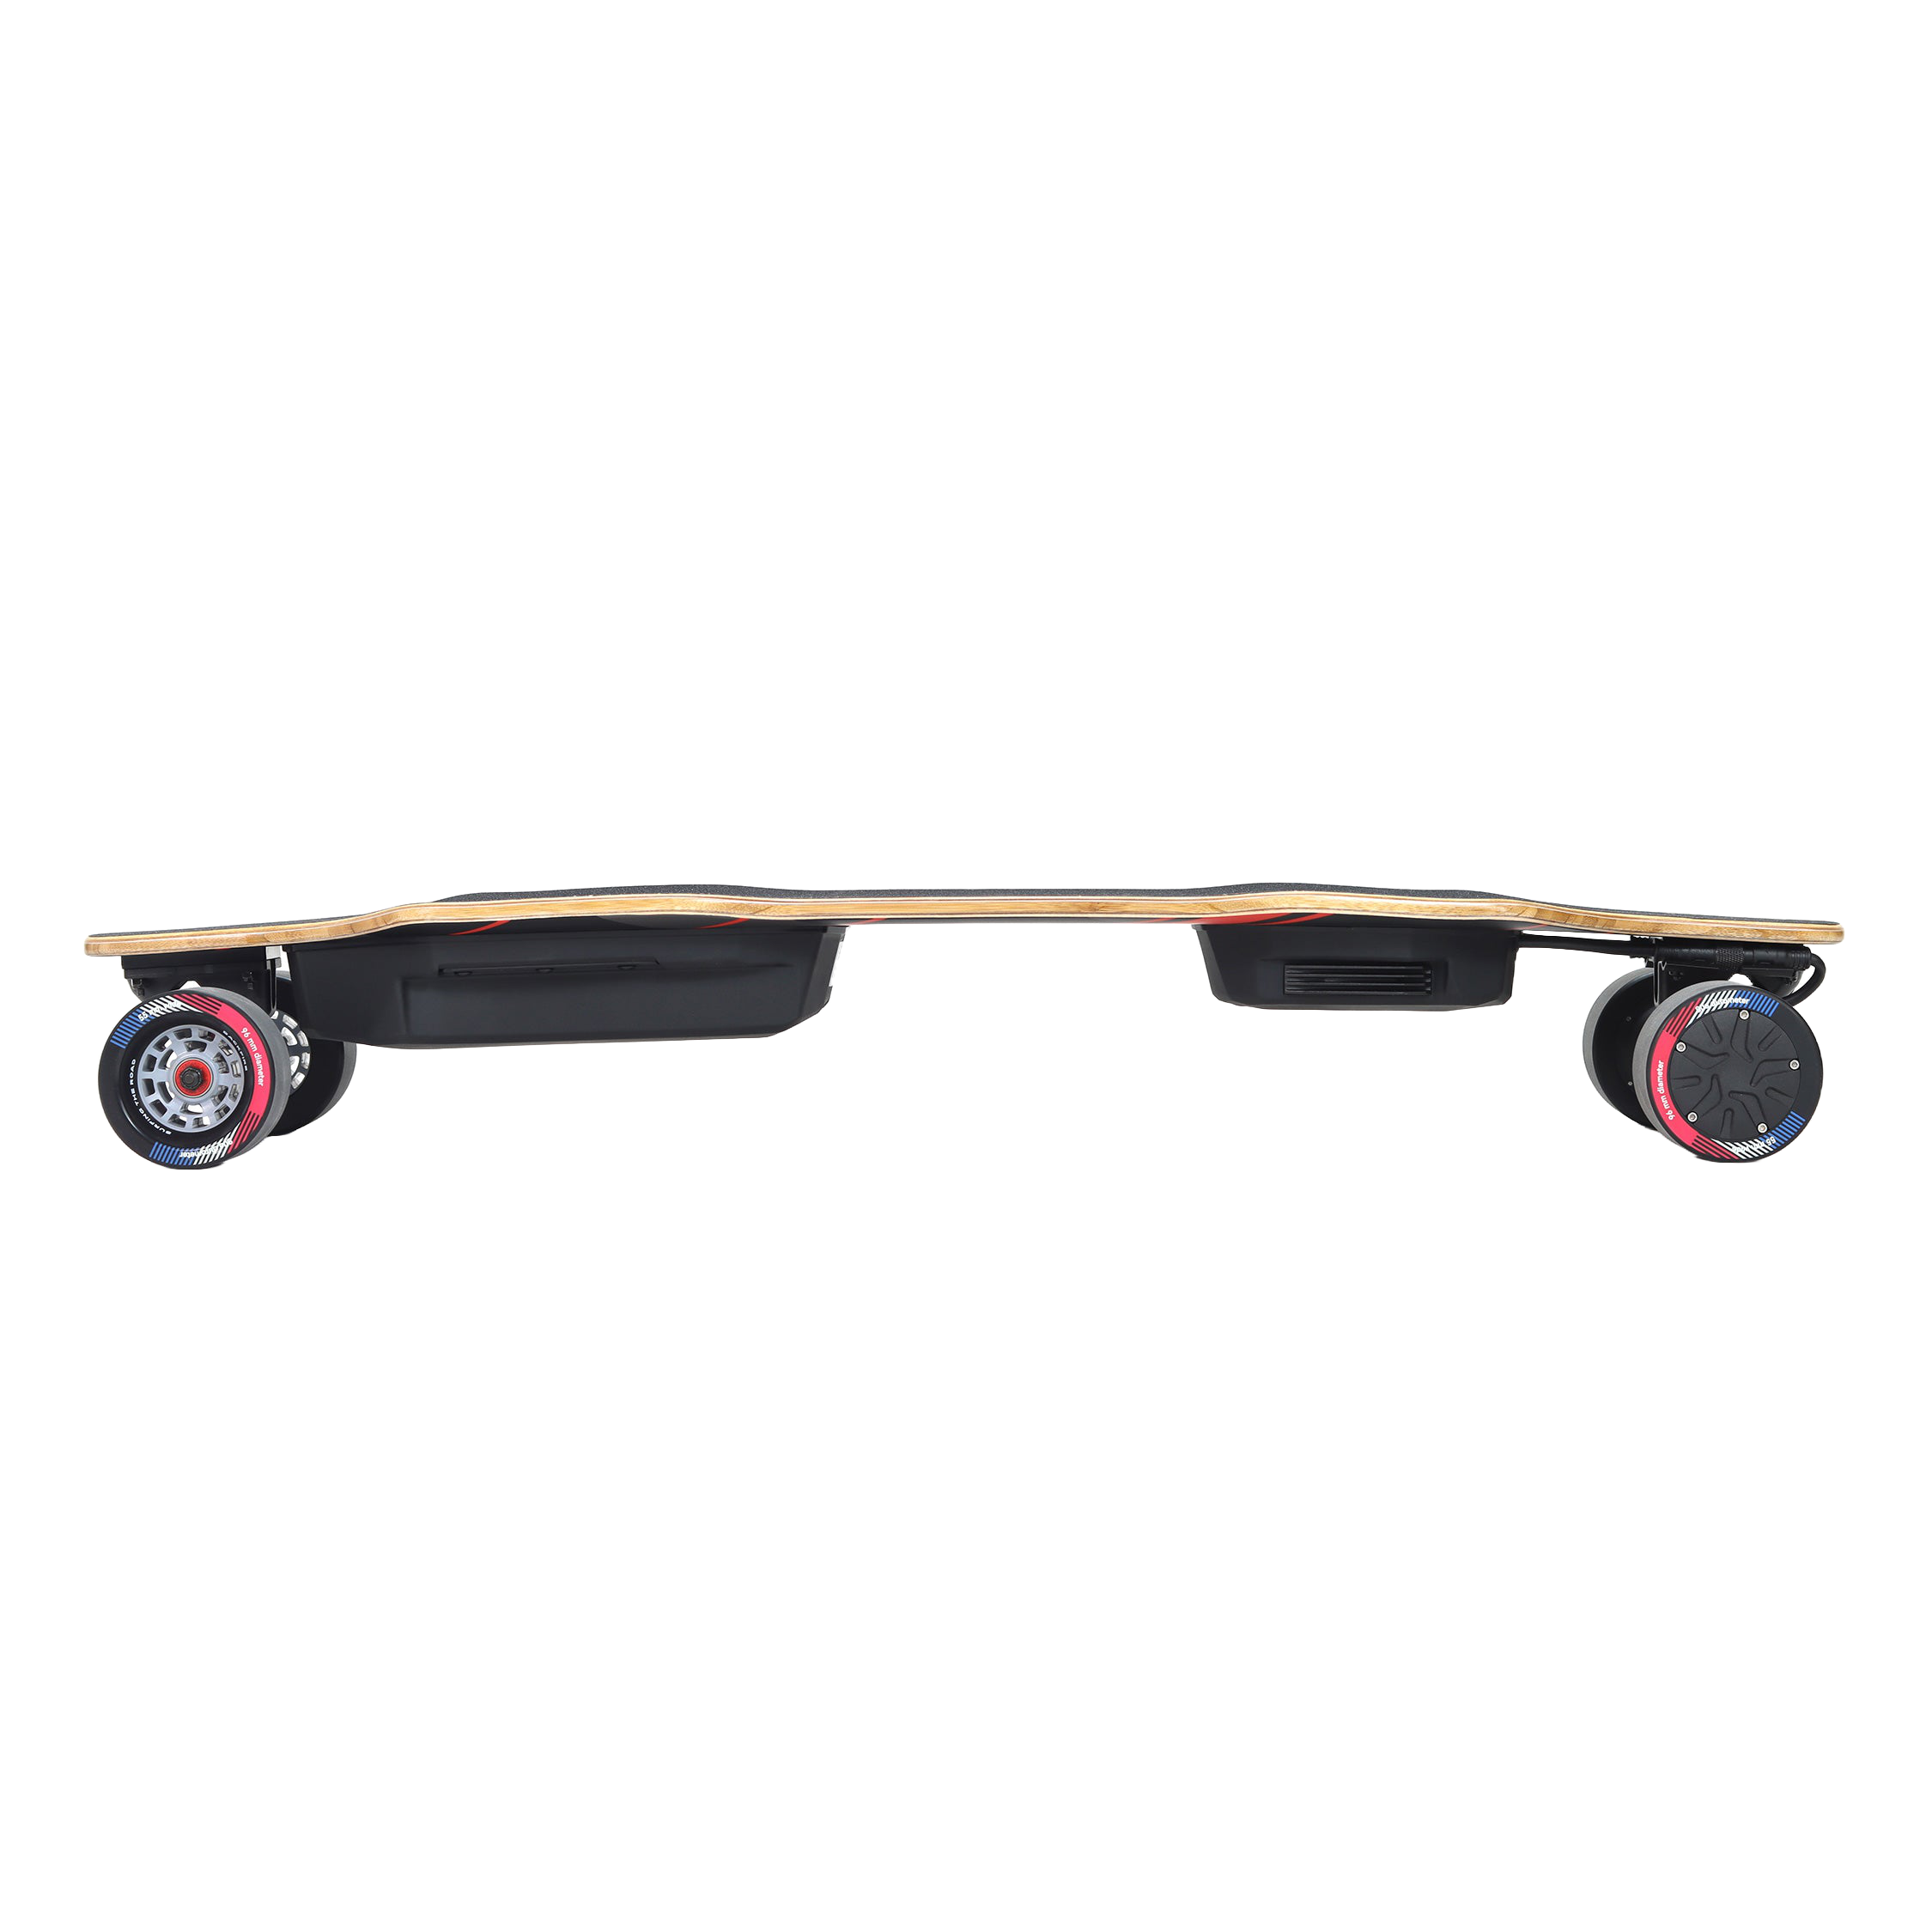
\includegraphics[width=0.48\linewidth]{obrazky-figures/brand-reviews/backfire-longboard.png}\hfill
    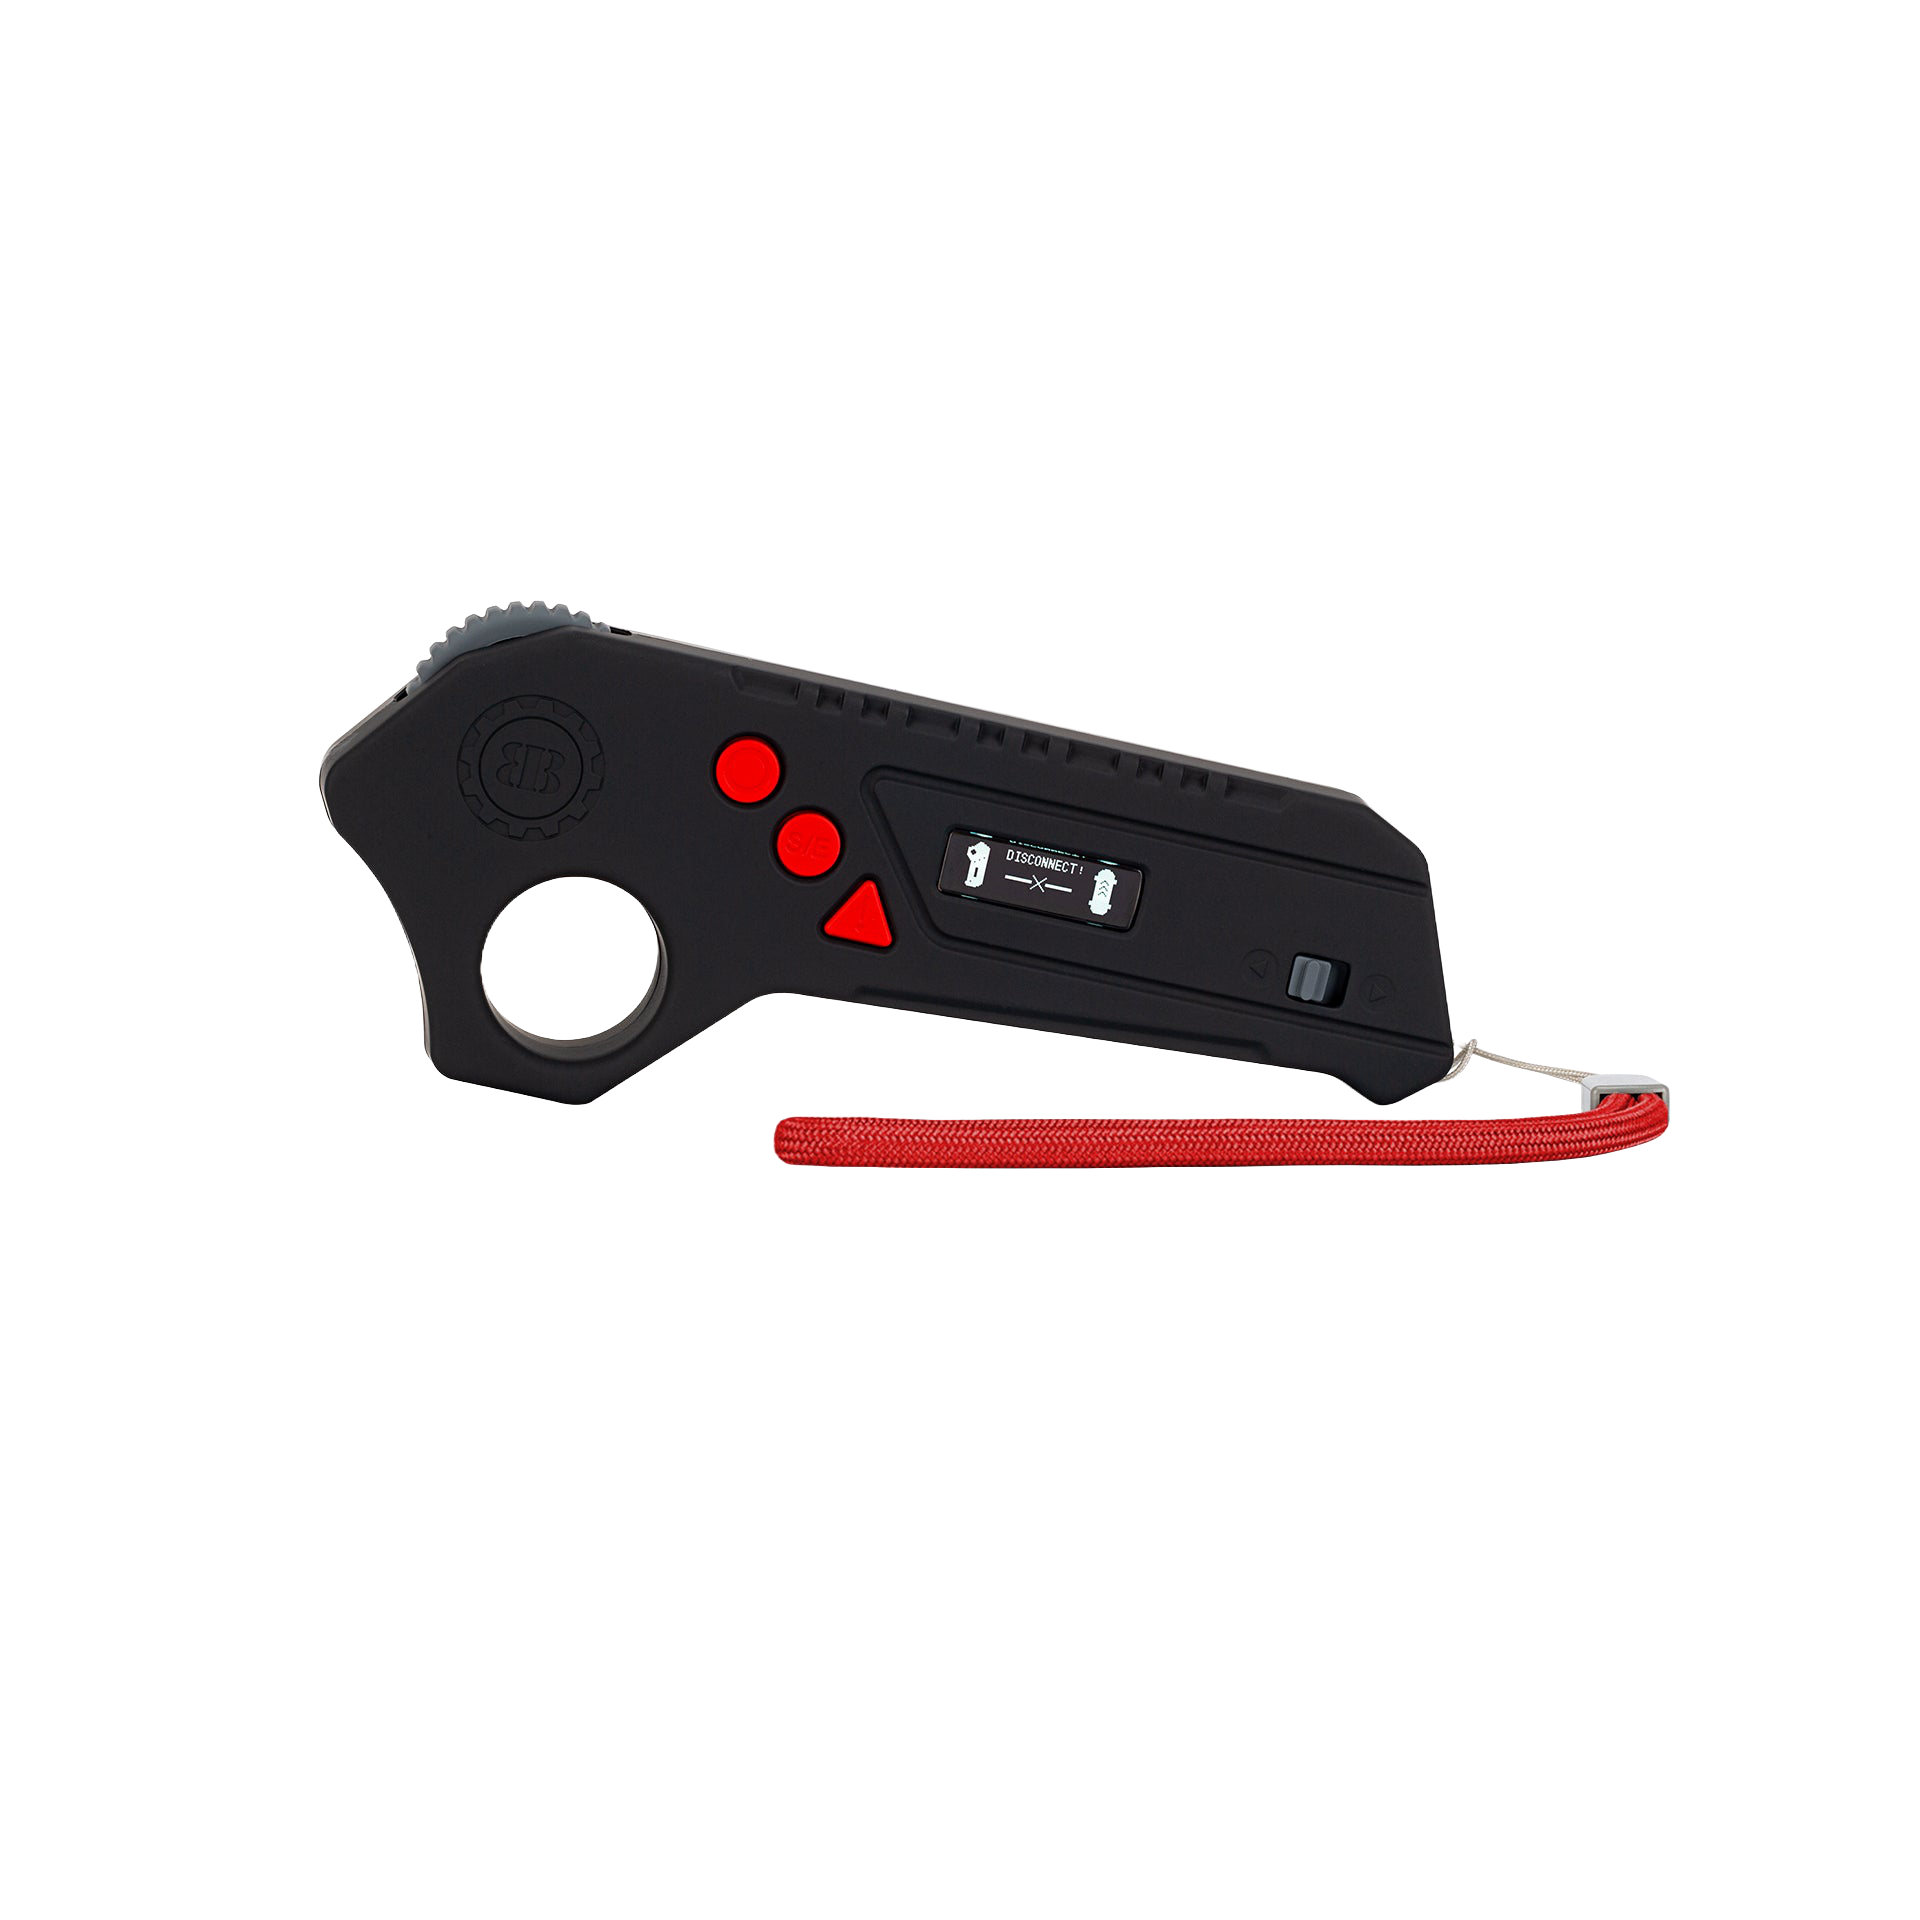
\includegraphics[width=0.48\linewidth]{obrazky-figures/brand-reviews/backfire-controller.png}
    \caption{Backfire G5 longboard a ovládač\cite{Backfire}}\label{fig:backfire}
\end{figure*}

Aplikácia Backfire, dostupná pre iOS a Android mobilné zariadenia, slúži najmä na zdieľanie informácii o~jazdách a komunikáciu s~komunitou.
Sledovanie stavu dosky a jej konfigurácie je veľmi limitovaná.
Umožňuje len základné nastavenia.
Aplikácia je však vhodná pre užívateľov, ktorí chcú zdieľať svoje jazdy a komunikovať s~ostatnými jazdcami.\cite{Backfire}

\section{Halo}
Halo je britský výrobca elektrických longboardov a hoverboardov.
Ponúka na výber len zopár modelov elektrických longboardov, ktoré sú však vysoko špecializované a prispôsobené pre náročných jazdcov.
Longboardy používajú Direct drive motory, ktoré sú spojené priamo s~kolesami a umožňujú vyšší výkon a efektivitu.
Halo sa zameriava na výkon a kvalitu, čo sa odráža aj na vyššej cene.
Obmedzený výber modelov a príslušenstva môže byť nevýhodou pre užívateľov, ktorí hľadajú špecifické a robustné zariadenia.

\begin{table}[h]
    \centering
    \begin{tabular}{|l|l|}
        \hline
        \textbf{Parameter} & \textbf{Hodnota} \\ \hline
        Maximálna rýchlosť & 42 km/h \\ \hline
        Dojazd & 41 km \\ \hline
        Maximálne stúpanie & 25\% \\ \hline
        Počet jazdných režimov & 3 \\ \hline
        Akumulátor & Li-Ion 345.6 Wh, 10S4P \\ \hline
        Typ akumulátorového článku & LG 18650, 2400 mAh \\ \hline
        Doba nabíjania & 4--5 h \\ \hline
        Výkon motora & 2x 1600 W \\ \hline
        Typ pohonu & Direct drive \\ \hline
        Hmotnosť dosky & 10.4 kg \\ \hline
        Cena & \$1797 ($\approx$1740 €) \\ \hline
    \end{tabular}
    \caption{Parametre elektrického longboardu Halo Beast (Obrázok~\ref{fig:halo})~\cite{Halo}}\label{tab:halo}
\end{table}

Halo longboardy majú ovládač s~otočným kolečkom na zrýchlenie a brzdenie.
Multifunkčné tlačídlo na zapnutie a vypnutie ovládača, umožňuje zapnúť funckiu na udržiavanie konštantnej rýchlosti.
Tlačidlo na prepínanie jazdných režimov je spolu s~tlačidlom napájania umiestnené na strane ovládača.
Na ovládači je tiež možné sledovať stav batérie dosky a ovládača, rýchlosť, prejdenú vzdialenosť a akutálny režim jazdy pomocou dispeja.

\begin{figure*}[h]
    \centering
    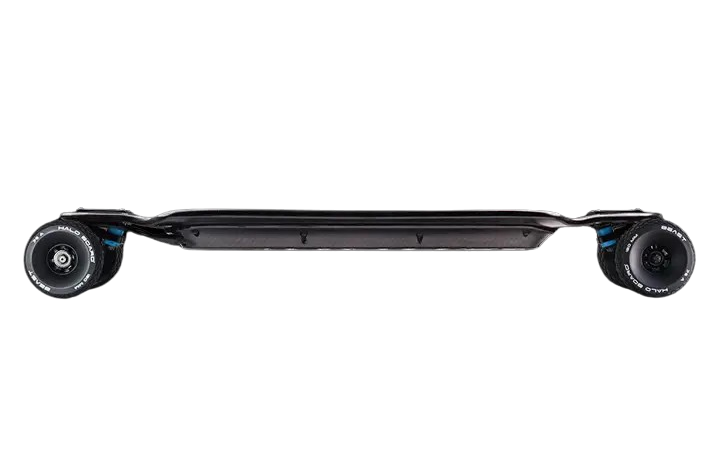
\includegraphics[width=0.48\linewidth]{obrazky-figures/brand-reviews/halo-longboard.png}\hfill
    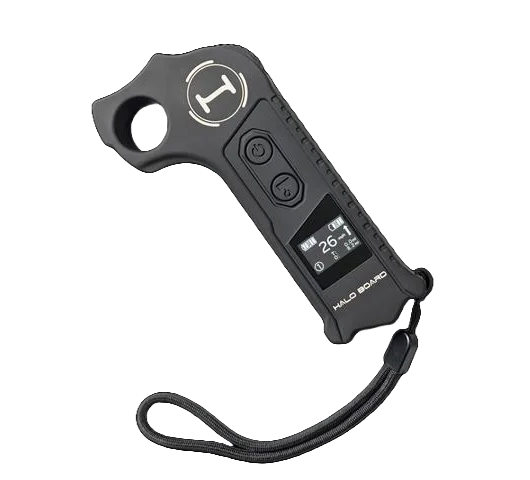
\includegraphics[width=0.48\linewidth]{obrazky-figures/brand-reviews/halo-controller.png}
    \caption{Halo Beast longboard a ovládač\cite{Halo}}\label{fig:halo}
\end{figure*}

Značka Halo neponuká pre svoje longboardy mobilnú aplikáciu pre sledovanie a konfiguráciu dosky.\cite{Halo}

\chapter{Návrh požiadaviek}\label{navrh}
Na základe analýzy trhu boli určené požiadavky na návrh elektrického longboardu s~elektrickým pohonom.
V~nasledujúcich podkapitolách sú podrobne popísané požiadavky na hardvérové a softvérové prostriedky, ktoré budú použité na zhotovenie prototypu.
Okrem návrhu na zhotovenie prototypu je tiež potrebné zvážiť možnosti testovania a overovania vlastností výrobku.

%TODO požiadavky / ciele práce

\section{Návrh hardvérových prostriedkov}
Zo získaných informácií a požiadaviek vyplýva, že jeho konštrukciu by mali tvoriť nasledujúce zariadenia a komponenty zakreslené na obrázku~\ref{fig:blokova_schema}.

\begin{figure}[h]
    \centering
    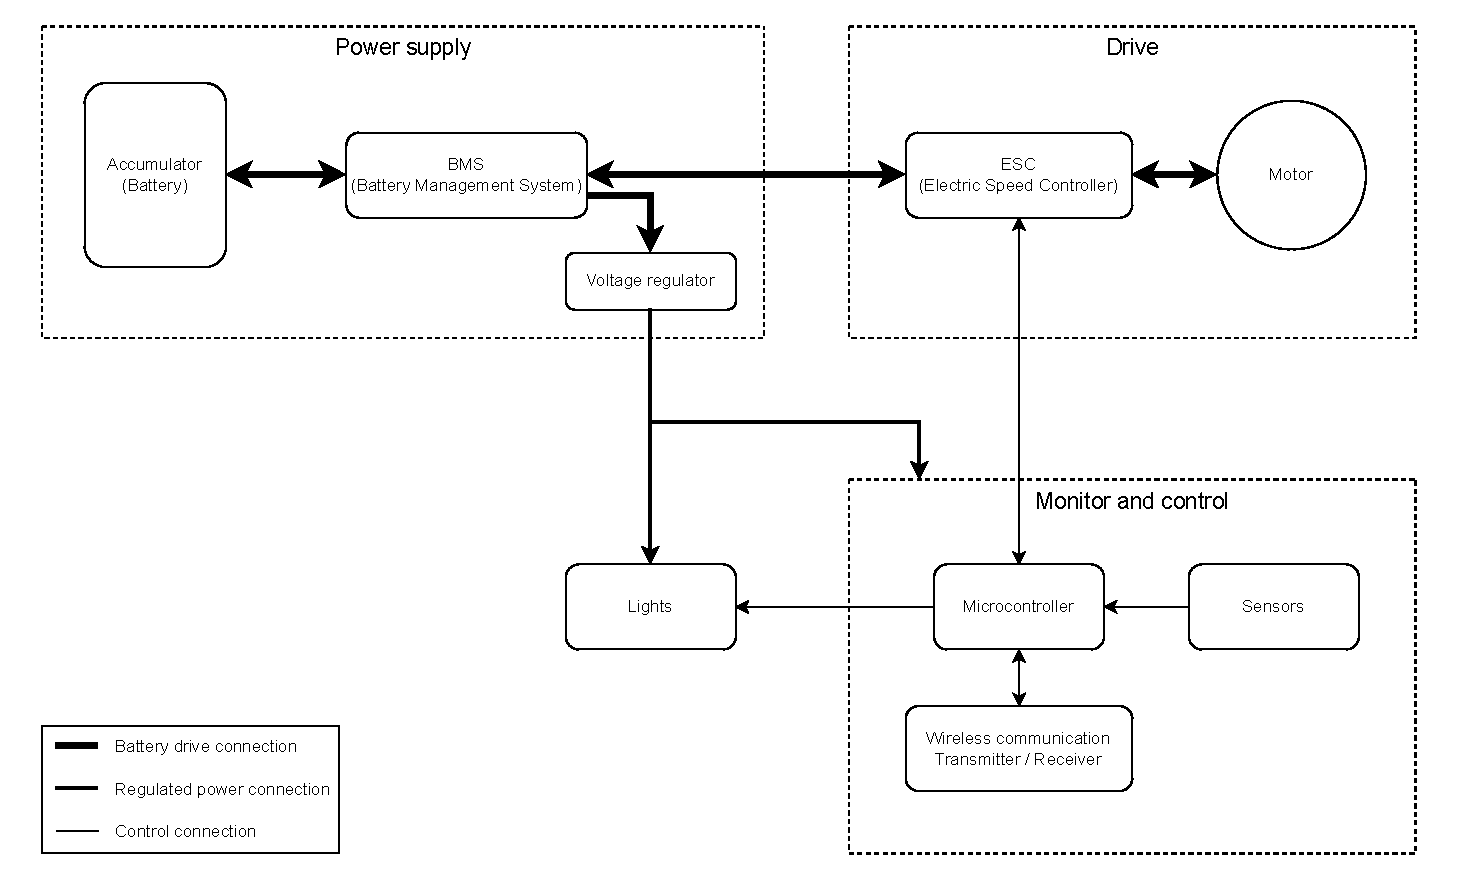
\includegraphics[width=1\textwidth]{obrazky-figures/block-diagram.pdf}
    \caption{Bloková schéma prepojenia všetkých komponentov}\label{fig:blokova_schema}
\end{figure}

Na obrázku sa nachádzajú ucelené bloky pre napájanie, pohon, ovládanie a monitorovanie, ktoré sú vzájomne prepojené.
Každý blok obsahuje viacero komponentov, ktoré spolu komunikujú alebo sa navzájom ovplyvňujú, a tak spolupracujú na dosiahnutí požadovaných vlastností výrobku.

\subsection{Pohon}
Pohon elektrického longboardu tvorí elektromotor a ESC (Electric speed controller).
U~väčšiny značiek je pohon zložený z~dvojice elektromotorov a ESC.
Je možné nájsť aj menej bežné modely s~pohonom na jedno koleso alebo s~pohonom na všetky štyri kolesá.
Pre prototyp bude zvolený pohon s~dvojicou elektromotorov.

Podľa analýzy trhu je najčastejšie používaným typom pohonu Belt drive.
Ďalší typ pohonu s~Hub motorom je tiež veľmi populárny, ale disponuje menším výkonom.
Direct drive nie je veľmi rozšírený a je používaný len niekoľkými značkami, pretože môže cenovo prevýšiť spomenuté typy pohonov.
Pre prototyp bude zvolený Belt drive, pretože je najjednoduchší na implementáciu a má dostatočný výkon pre požadované vlastnosti, ktoré je možné ľahko ladiť.
Prevod pohonu bude zabezpečený remeňom, ktorý bude spojený s~motorom a kolesom.
Motor bude umiestnený na spodnej strane dosky a bude poháňať zadné koleso.

Typ motoru bude BLDC motor s~vysokým výkonom a efektivitou.
Motory určené na pohon elektrických longboardov sú schopné pracovať s~akumulátormi zloženými zo 4 až 12 seriovo zapojených článkov.
Motor s~výkonom 2500--3500~W bude dostatočný pre dosiahnutie požadovanej rýchlosti a umožní jadzu aj v~náročnejších podmienkach.
BLDC motory s~integrovanými Hallovými senzormi, umožňia presnejšie riadenie a monitorovanie otáčok motora.\cite{TorqueBoards}

\bigskip

ESC je hlavným riadiacim a komunikačným prvkom pohonu.
Výber ESC je viac závislý od požadovaných komunikačných protokolov a možností konfigurácie, ako od výkonu.
Najvhodnejším ESC pre elektrický longboard je VESC (Vedder's Electronic Speed Controller), ktorý je adaptovaný viacerým výrobcami.
Všetky varianty VESC majú podobné vlastnosti a umožňujú konfiguráciu systému podľa požiadaviek užívateľa.
ESC s~maximálnym kontinuálnym prúdom aspoň 40~A~bude dostatočný pre dodávanie potrebného výkonu motorom.
Okrem výberu samotného ESC je dôležité ho aj správne nastaviť a kalibrovať, aby zabezpečil bezproblémovú prevádzku celého systému.\cite{VESC}

\bigskip

Brzdenie je podstatná vlastnosť pohonu, ktorá zabezpečuje bezpečnú prevádzku.
Ako elektronická brzda bude využitá rekuperácia energie, ktorá umožňuje dobíjať akumulátor pri brzdení.
V~rámci prieskumu alternatívnych spôsobov brzdenia bola zvážená aj mechanická brzda, ktorá by zabezpečila bezpečné brzdenie v~prípade výpadku elektronického systému.
Problém s~mechanickou brzdou je v~jej požadovanom umiestnení na zadných kolesách, na ktorých sa už bude nachádzať elektrický pohon.
Vybavenie elektrického longboardu mechanickou brzdou, na doporučenie od europskej rady pre bezpečnosť v~doprave~\cite{CDV}, si vyžaduje navrhnutie vlastného riešenia, ktoré nie je súčasťou tejto práce.

\begin{figure}
    \centering
    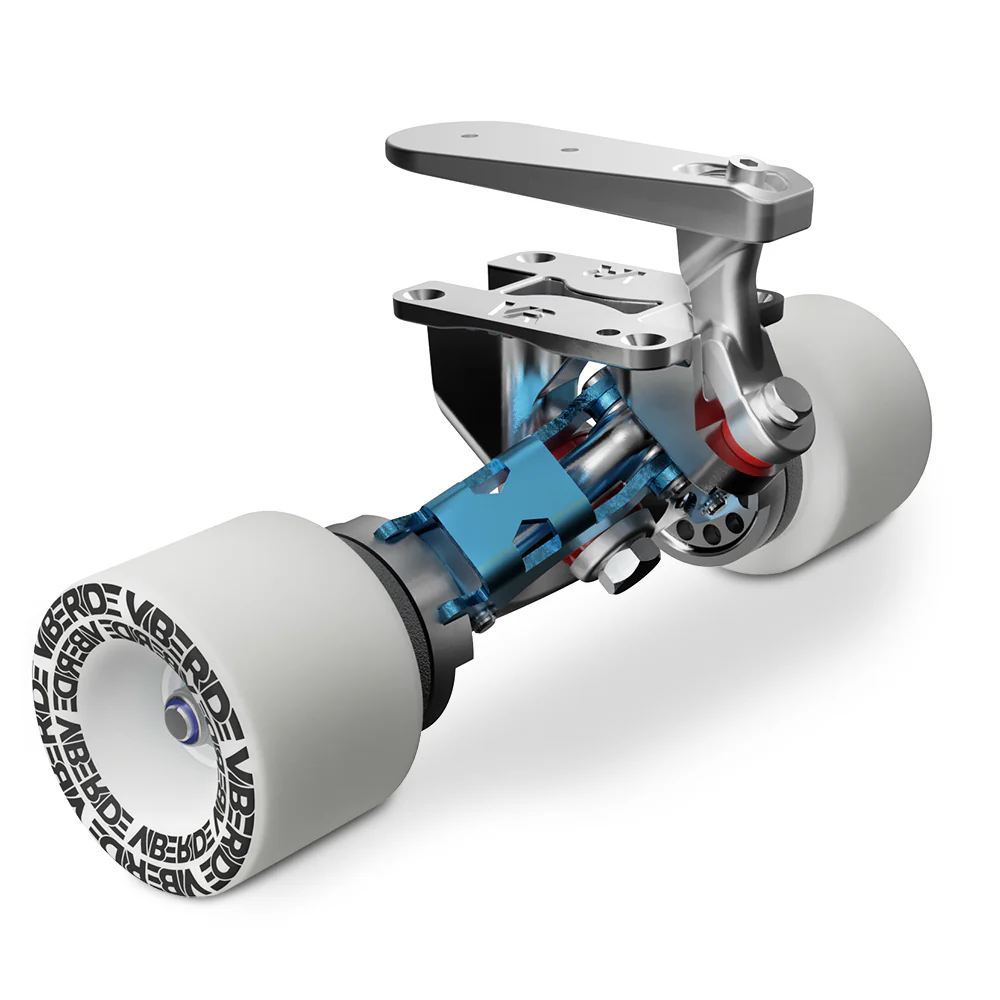
\includegraphics[height=8cm]{obrazky-figures/mechanic-brake.png}
    \caption{Mechanická brzda od značky Viberide\cite{Viberide}}\label{fig:mechanic-brake}
\end{figure}

\subsection{Napájanie}
Napájanie je kľúčovým prvkom elektrického longboardu.
Závisí od neho výkon, dojazd a bezpečnosť celého systému.
Pozostávať bude z~akumulátora, BMS a napäťového deliča.
Tieto komponenty, zabezpečia stabilné a bezpečné napájanie pre všetky komponenty.

Z~analýzy trhu vyplýva, že najčastejšie používaným typom je akumulátor zložený z~Li-Ion článkov.
Je možné ich ľahko kombinovať do väčších batérií s~vyššou kapacitou a napätím.
Z~pohľadu testovania a prototypovania systému postačia aj Li-Po akumulátory, ktoré sú bezpečnejšie a pracuje sa nimi jednoduchšie.
Ich kombinácia do väčších batérií vyžaduje len prepojenie článkov pomocou konektorov a pri spájaní pomocou pájky nie sú tak citlivé na tepelné poškodenie.
V~konečnom produkte sa však použijú Li-Ion akumulátory, ktoré umožnia nabíjanie vyšším prúdom. 
Taktiež je ich možné oveľa ľahšie integrovať do dizajnu dosky v~prípade skladania vlastného akumulátora.

Vyššieho dojazdu elektrického longboardu docielime navyšovaním kapacity akumulátora. 
Znamená to však aj zvýšenie hmotnosti a ceny celého systému.
Preto je dôležité zvoliť kompromis medzi dojazdom, hmotnosťou a cenou.
Akumulátor zložený z~2 a viac paralelne zapojených článkov zabezpečí dostatočný prúdový výkon pre elektromotory a zvýši dojazd.
Vyšší výkon motora dosiahneme zvýšením napätia akumulátora.
Je dôležité poznať maximálne limity celého systému, tak aby ani vysoké napätie nepoškodilo komponenty ktoré napája.
Z~uvedených parametrov vyplýva, že vhodným akumulátorom je Li-Ion akumulátor s~minimálným nominálnym napätím 36--37 V~--- 10 článkov zapojených v~sérii.

Na výber je niekoľko velkostí Li-Ion článkov a pri ich výbere je nutné zvážiť aj umiestnenie akumulátora na doske. 
Z~najčastejšie používaných článkov, 18650 a 21700, existuje viacero značiek a modelov, ktoré ponúkajú vhodné vlastnosti pre elektrický longboard.\cite{BatterySpaceTypes}
Pri priemernej spotrebe motora $\approx$20~A~a schopnosti zvládnuť nabíjací prúd aspoň 4~A, aby sa dosiahla kratšia doba nabíjania, je vhodné zvoliť článok s~minimálnou kapacitou 3500~mAh.
Dôležitým faktorom pri výslednom výbere článkov je okrem jej vlastností aj cena za Wh a dostupnosť na trhu.

\bigskip

BMS je nutným bezpečnostným prvkom pre akumulátor a užívateľa.
Voľba správneho BMS zabezpečí bezpečnú prevádzku celého systému a predĺži životnosť akumulátora.
Ochrana pred prebitím, podbitím, preťažením, prehriatím a skratom sú minimálne požiadavky pre BMS.
Výber BMS závisí od požiadovaných vlastností, ako je maximálny prúd a zapojenie článkov.
Pre akumulátor zložený z~10S článkov bude vhodný BMS s~minimálnym vybíjacím prúdom 40~A~a minimálnym nabíjacím prúdom 20~A, tak aby pri jazde nedochádzalo k~neočakávanému vypnutiu systému.
Iné BMS s~možnostou balancovania článkov je možné, v~prípade elektrického longboardu, pripojiť k~akumulátoru len externe pri priebežnej kontrole akumulátoru, nakoľko nie je nutné často balancovať články.

Okrem bezpečnostých funkcií majú niektoré BMS aj zahrnutý spínač obvodu a komunikačné rozhranie, ktoré umožňuje podrobné monitorovanie stavu akumulátora.
Tieto funkcie môžu zlepšiť bezpečnosť celého systému a pômôcť pri diagnostike problémov.

\bigskip

Napäťový delič je potrebný pre zabezpečenie napájania pre všetky komponenty, ktoré nedokážu pracovať pri vyššom napätí.
Zložený bude z~DC-DC konvertora, ktorý bude znižovať akumulátorove napätie na požadovanú hodnotu. 

\subsection{Ovládanie a monitorovanie}

Hlavným prvkom ovládania a monitorovania elektrického longboardu je mikrokontrolér.
Mikrokontrolér bude zabezpečovať riadenie elektromotorov cez komunikáciu s~ESC, zber a spracovanie dát zo senzorov a komunikáciu s~užívateľom.
Na naplnenie požiadaviek bude zvolený mikrokontrolér z~rady ESP32, ktorý je vhodný pre aplikácie s~vyššími požiadavkami na komunikačné protokoly a rozhrania.

Mikrokontroléry z~rady ESP32 sú moderné mikrokontroléry s~vysokým výpočetným výkonom a podporou komunikačných rozhraní Wi-Fi a Bluetooth.
Takže sú vhodné na bezdrôtovú komunikáciu s~mobilným zariadením alebo ovládačom bez dodatočných modulov, ktoré využívajú tieto technológie.
Obsahujú viacero analógových a digitálnych vstupno-výstupných pinov, takže postačia na pripojenie senzorov a komponentov cez štandartne používané protokoly a rozhrania ako I2C, SPI a UART\@.
V~prípade ak senzor alebo iný modul nevyužíva komunikačné rozhranie, je možné využiť na jeho ovládanie interné prevodníky ADC a DAC alebo generátor signálu PWM\@.
Na uloženie programu a dát na ESP32 poslúži interná pamäť SRAM (Static Random Access Memory) s~kapacitou 520~kB alebo v~externá Flash pamäť s~kapacitou 4--16~MB\@.
Flash pamäť sa využije aj na OTA (Over-the-Air) aktualizácie firmvéru, čo zjednoduší aktualizáciu systému bez nutnosti fyzického pripojenia k~počítaču.\cite{Espressif}

\begin{figure}
    \centering
    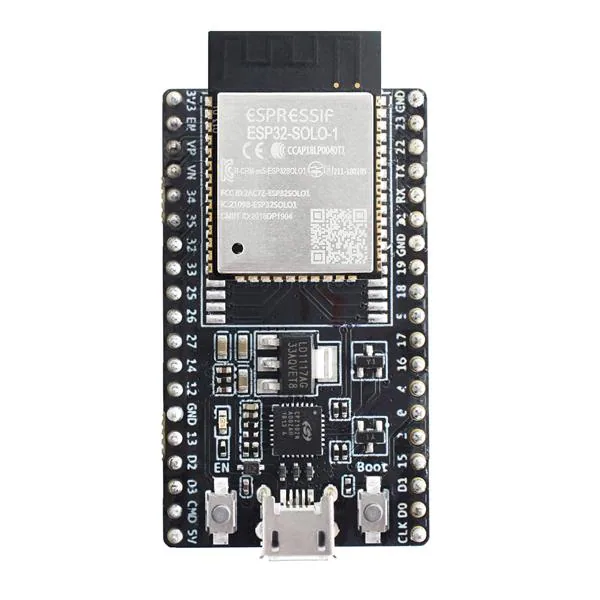
\includegraphics[height=8cm]{obrazky-figures/esp32-devkit.png}
    \caption{Vývojová doska ESP32-DevKitC s~mikrokontrolérom ESP32\cite{Espressif}}
\end{figure}

Pri komunikácii mikrokontroléra s~ESC bude mikrokontrolér plniť úlohu prostredníka.
ESC bude cez komunikačné rozhranie UART prijímať príkazy od mikrokontroléra a poskytovať informácie o~svojom stave.
Na užívatelské vstupy bude mikrokontrolér aplikovať rôzne algoritmy, aby sa predišlo nebezpčným situáciám a zlepšila ovládateľnosť.
Hodnoty z~akcelerometru a gyroskopu budú ukladané do pamäte mikrokontroléra a pribežne využívané na adaptáciu jazdných vlastností, ale aj na vyhodnocovanie kritických situácií.
Longboard spomalí alebo aj zastaví, ak sa zistí náraz alebo pád.
Vhodným komponentom, ktorý kombinuje akcelerometer, gyroskop a magnetometer je IMU (Inertial Measurement Unit).
IMU bude umiestnený spolu s~ostatnými komponentmi na spodnej strane dosky.

Umiestnenie tepelného senzora na akumulátor, motor alebo ESC umožňí monitorovať teplotu týchto kritických komponentov.
Tieto hodnoty budú spolu s~ostatnými dátami optimalizovať výkon systému.
Optimalizácia výkonu systému v~závislosti od teploty zvýši bezpečnosť a životnosť zariadenia.

Na zvýšenie bezpečnosti pri jazde v~noci bude na doske umiestnené predné a zadné osvetlenie.
Ideálnou voľbou bude LED osvetlenie, ktoré vďaka nízkej spotrebe nebude zbytočne zaťažovať akumulátor.

\subsection{Návrh ovládača}

Rovnako ako pri elektrickom longboarde, aj pri ovládači je mikrokontrolér riadicim prvkom.
Na ovládači bude taktiež zvolený mikrokontrolér z~rady ESP32.
Umožňuje to využiť rovnaké komunikačné rozhrania s~longboardom a v~prípade aktualizácie firmvéru aj pripojenie s~mobilným zariadením.

Pri návrhu ovládania je dôležité zvoliť vhodné komponenty, ktoré zabezpečia pohodlné a bezpečné ovládanie elektrického longboardu.
Z~prieskumu trhu vyplýva, že najpoužívanejším typom ovládania je ovládanie s~otočným kolečkom na zrýchlenie a brzdenie.
Toto riešenie ponúka jemnú reguláciu rýchlosti a ovládanie brzdenia v~jednom ovládacom prvku.
Pre pokročilých užívateľov je však vhodnejšie ovládanie s~lineárnymi spínačmi, ktoré umožňujú rýchlejšie reakcie na zmeny rýchlosti.
Ovládač s~otočným kolečkom a lineárnym spínačom je ideálnym riešením, pretože kombinuje výhody oboch typov ovládania.
Niekoľko spôsobov ovládania umožní užívateľovi zvoliť si najvhodnejší spôsob ovládania pre jeho štýl jazdy s~využitím ukazováka alebo palca.

\begin{figure}
    \centering
    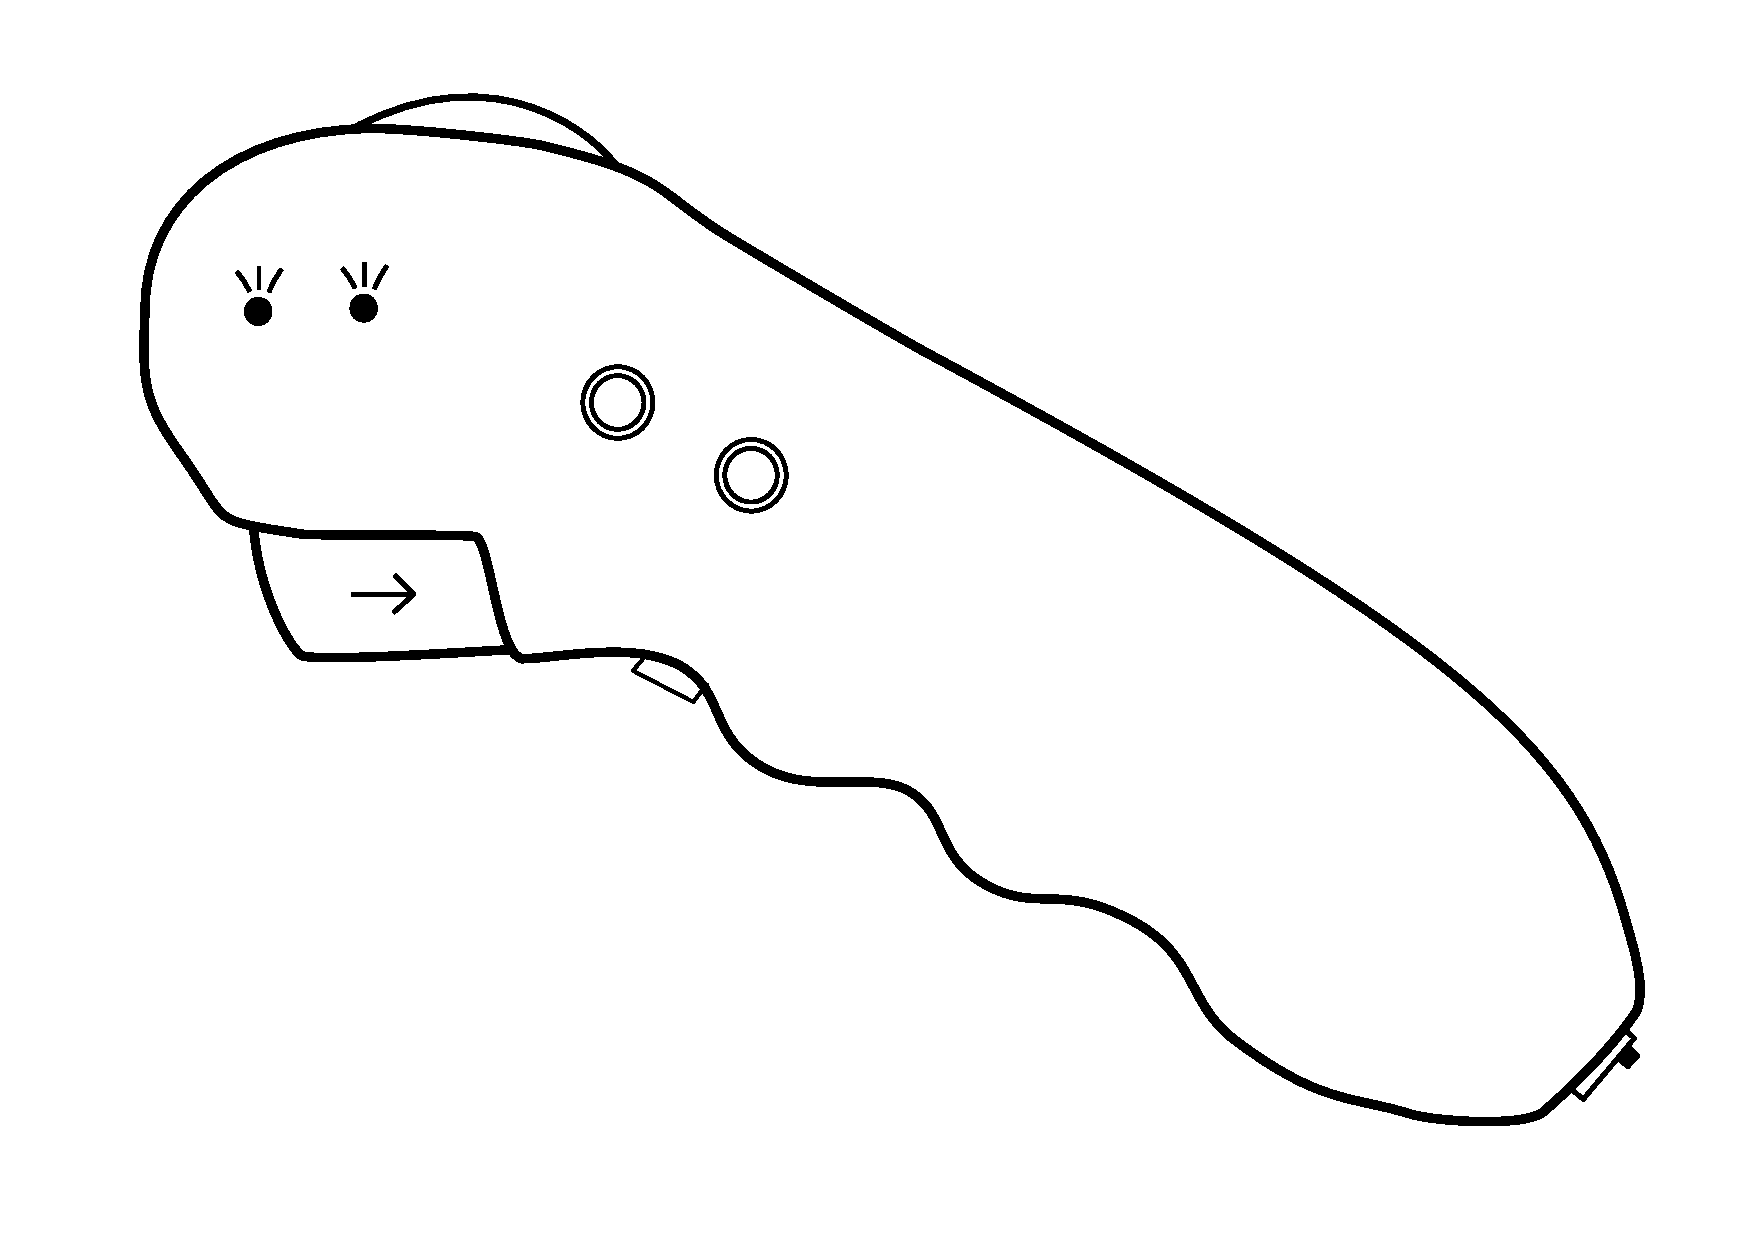
\includegraphics[height=10cm]{obrazky-figures/controller.pdf}
    \caption{Návrh ovládača s~otočným kolečkom a lineárnym spínačom}\label{fig:remote-control}
\end{figure}

Návrh ovládača obsahuje aj tlačidlo na vnútornej strane, ktoré musí užívateľ stlačiť a držať pre aktiváciu pohonu alebo držanie konštantnej rýchlosti.
Tlačidlo na zapnutie/vypnutie osvetlenia a tlačidlo na prepínanie jazdných režimov bude umiestnené na bočnej strane ovládača.
Na spodnej strane sa bude nachádzať vypínač a USB-C konektor na nabíjanie akumulátora ovládača. 

Signalizačné LED diódy na ovládači budú informovať užívateľa o~stave batérie ovládača a longboardu, prípadne o~stave spojenia s~elektrickým longboardom.
Návrh ovládač neobsahuje displej, pretože všetky ostatné informácie bude možné zobraziť na mobilnom zariadení.

\section{Návrh softvérových prostriedkov}

Softvérové prostriedky tvorí aplikácia pre mobilné zariadenie a firmvér pre mikrokontroléry ESP32 v~elektrickom longboarde a ovládači.
Ich vzájomná komunikácia musí byť spoľahlivá a rýchla, aby zabezpečila bezproblémovú prevádzku celého systému.

\subsection{Programovanie mikrokontroléra}

Na programovanie mikrokontroléra ESP32 existujú dve hlavné platformy: Arduino IDE a ESP-IDF (Espressif IoT Development Framework).
Jednoduché programovanie mikrokontroléra je možné pomocou vývojového prostredia Arduino IDE.
Má zjednodušené ovládanie a ponúka množstvo knižníc pre rôzne senzory a komponenty.
Arduino IDE je veľmi populárne medzi začiatočníkmi a umožňuje rýchle vytvorenie funkčného prototypu.\cite{Arduino}
Pri vývoji komplexnejších aplikácií je však vhodné použiť ESP-IDF
ESP-IDF je vývojový nástroj od spoločnosti Espressif, ktorá vyvíja mikrokontroléry ESP32.
Tento nástroj poskytuje viac možností pre konfiguráciu a umožňuje využiť všetky vlastnosti mikrokontroléra ESP32.
Vývoj v~ESP-IDF je náročnejší, ale pomáha vytvoriť robustný a optimalizovaný systém.\cite{EspressifIDF}
Pre vývoj firmvéru pre elektrický longboard a ovládač bude na základe týchto vlastností vhodnejšie použiť ESP-IDF.

Vývoj firmvéru v~C/C++ jazyku dovoľuje využiť dostupné knižnice pre zjednodušenie vývoju komunikácie s~ostatnými modulmi a senzormi. 
Rovnako aj VESC má firmvér s~otvoreným zdrojovým kódom v~C.
Takže je možné vďaka knižniciam, komunikovať s~VESC cez UART a získať tak informácie o~stave priamo z~VESC senzorov.

\subsection{Komunikačný protokol}

Mikrokontrolér v~elektrickom longboarde bude komunikovať s~mikrokontrolérom v~ovládači alebo s~mobilným zariadením.
Aby zariadenia mohli vzájomne komunikovať, je potrebné navrhnúť komunikačný protokol, ktorý bude zabezpečovať bezpečný a spoľahlivý prenos dát.
Je vhodné aby komunikačný protokol bol jednoduchý a mal určenú formu odosielaných dát.
Prenášať sa budú len dáta a kontrolné hodnoty packetu ako napríklad CRC (Cyclic Redundancy Check) kód alebo dĺžka packetu.
Sémantika jednotlivých dát bude závisieť od typu packetu.

\subsection{Návrh mobilnej aplikácie}

Mobilná aplikácia musí umožňovať užívateľovi okrem sledovania stavu elektrického longboardu a jeho konfigurácie aj možnosť náhrady ovládača.
Preto je potrebné navrhnúť aplikáciu na mieru, ktorá bude obsahovať viacero obrazoviek pre zobrazenie dát a možností ovládania.
Na trhu neexistuje žiadna aplikácia, ktorá by umožňovala náhradu ovládača a ich počet, ktoré umožňujú sledovanie stavu elektrického longboardu, je veľmi nízky.

Úvodná obrazovka bude obsahovať ako hlavnú možnosť prepojenie s~elektrickým longboardom a následného ovládania.
Po úspešnom prepojení budú zobrazené aj aktuálne dáta z~elektrického longboardu ako napríklad rýchlosť a stav batérie.
Ovládanie zrýchlenia a brzdenia bude pomocou ovládacích prvkov na celej oblasti obrazovky.

Jednou z~ostatných obrazoviek bude obrazovka pre konfiguráciu elektrického longboardu.
Na tejto obrazovke bude možné meniť jazdné režimy a ich nastavenia.
Konfigurácia týchto dát bude uložená v~pamäti elektrického longboardu a pri spojení s~ním budú tieto dáta načítané.
Súčasťou bude aj zobrazenie ostatných menej dôležitých dát o~elektrickom longboarde.
Zobrazené dáta budú aktualizované v~reálnom čase a ich ukladanie do pamäte mobilného zariadenia umožní neskôr ich analýzu.

Okrem konfigurácie jazdných vlastností longboardu je dôležité aj nastavenie samotnej aplikácia a jej komponentov.
Na obrazovke s~nastaveniami bude možné meniť vlastnosti aplikácie, konfigurovať bezdrôtové spojenie a aktualizovať firmvér mikrokontrolérov.

%TODO: wireframe mobilnej aplikacie

%\section{Zhrnutie aktuálneho stavu}\label{aktualny_stav}

%\chapter{Implementácia}\label{implementacia}

%linear trigger 
%https://www.ti.com/lit/ml/slyp837/slyp837.pdf?ts=1736532181420&ref_url=https%253A%252F%252Fwww.google.com%252F

%WROOM32
%https://lastminuteengineers.com/esp32-wroom-32-pinout-reference/


%crc code
%https://www.sunshine2k.de/articles/coding/crc/understanding_crc.html

%\chapter{Testovanie}\label{testovanie}

%\chapter{Závěr}\label{zaver}

%zhodnotenie cieľov práce
%cenové zhodnotenie 

%===============================================================================

% Pro kompilaci po částech (viz projekt.tex) nutno odkomentovat
%\end{document}
